\lhead{Progress Report}
\chapter{Progress Report}
\label{ProgressReport}

	The following progress report aims to provide a summary of the activities to date, the overall status of the project, as well as remaining work which will need to be completed by the end of the thesis period. In the outset of this section, a list of implemented Gaussian process models are listed, each of which will be expanded with results and figures. %In the outset of this section, I will begin by identifying the major problems which need to be addressed. I will then proceed by discussing the implemented solutions as well as those which will be implemented at a later stage.
	
	This report will focus on the environment modeling aspect, with some remarks on the path planning aspect of this project.

	\section{Gaussian Process Models}
	\label{ProgressReport:GaussianProcessModels}
	
		The environment modeling problem relies heavily on both the regression and classification technique of Gaussian process models. This section aims to present the work that has been done for building these models.
		
		Currently, the following Gaussian Process models have been implemented.
		
		\begin{itemize}
			\item Regression
			\item Multi-Task Regression
			\item Binary Classification
			\item Multi-Class Classification (One v.s. All)
			\item Multi-Class Classification (All v.s. All)
			\item Non-Stationary Kernels for all of the above
		\end{itemize}
		
		\subsection{Regression}

			Gaussian process regression can be split into two parts - single-task regression and multi-task regression. The single-task regression is the standard GP regression which is the underlying model for almost all of the other GP models, even for GP classification models. The multi-task version extends the single-task regression model to capture the covariance and hence relationship between multiple outputs, or \textit{tasks}, so that the different tasks can help each other in prediction under scarce training data.
			
			\subsubsection{Single-task Regression}
			
				The single-task regression presented here follows the standard implementations described in Rasmussen and Williams (2006) \cite{GaussianProcessForMachineLearning}. The model can handle any number of features in general. A simple one dimensional case is shown in \cref{ProgressReport:GaussianProcessModels:Figure:regression}.
				
				\begin{figure}[!htbp]
					\centering
						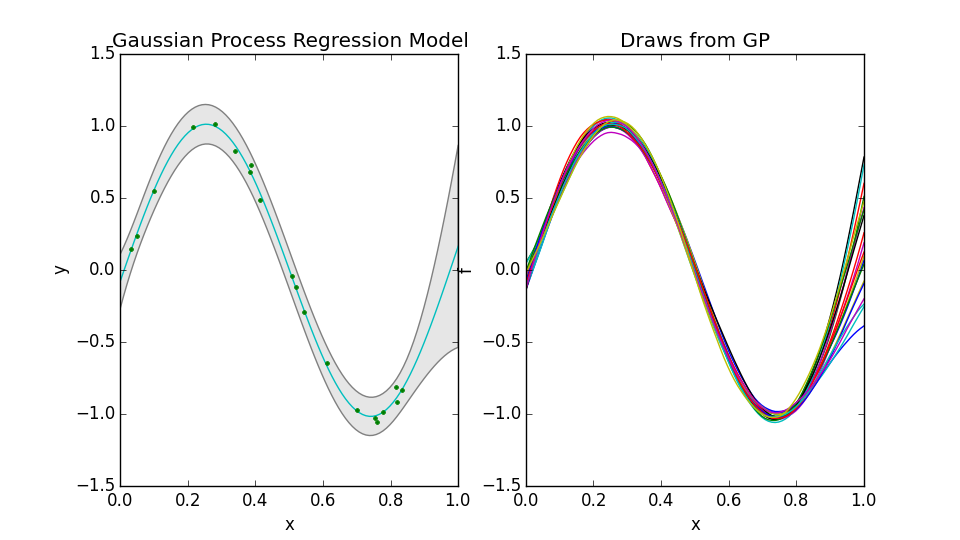
\includegraphics[width=0.9\textwidth]{Figures/Progress/regression.png}
					\caption{Gaussian Process Single-Task Regression \\
					Kernel Employed: Fusion of Squared Exponential Kernel and \matern 3/2 Kernel}
					\label{ProgressReport:GaussianProcessModels:Figure:regression}
				\end{figure}
						
				\FloatBarrier
				
				The model is trained to optimise the hyperparameters such that the log marginal likelihood, or log evidence, is maximised. Due to the Gaussian assumption, there exists an analytical form for the marginal likelihood of the observed data such that training can be done in reasonable time.
				
				If the hyperparameters are not learned properly, then the resulting model can experience various fault phenomenon. One of the most important problem is overfitting. In a GP setting, this can often happen when the learned length scale is too small. Figure \ref{ProgressReport:GaussianProcessModels:Figure:regressionbad} demonstrates a case where the length scale is artificially kept to 0.2, which is too small. Hence, the regression model experiences faster variations such that it overfits the data. It is evident from the GP draws that the correlation between neighboring points decreases much faster than before.
					
				\begin{figure}[!htbp]
					\centering
						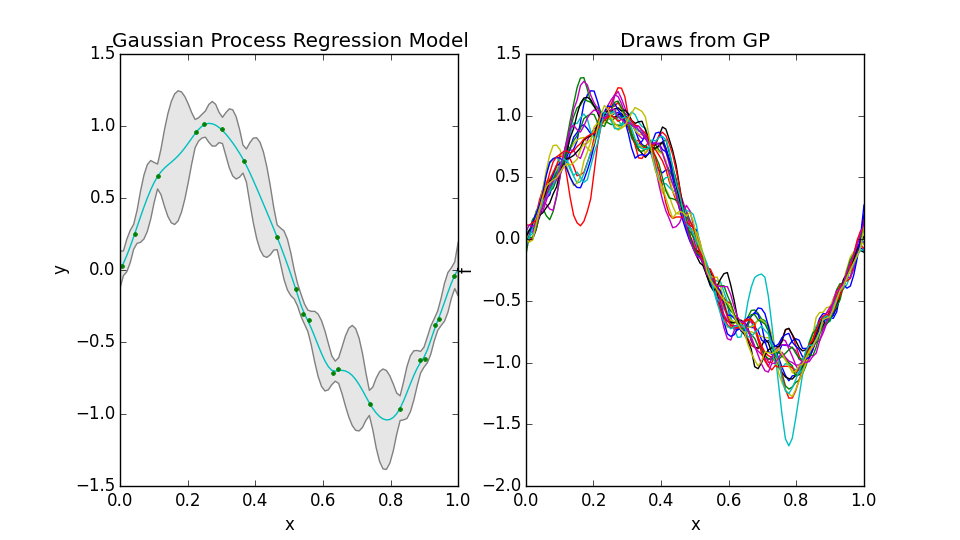
\includegraphics[width=0.9\textwidth]{Figures/Progress/regressionbad.png}
					\caption{Gaussian Process Single-Task Regression: Incorrect Length Scale}
					\label{ProgressReport:GaussianProcessModels:Figure:regressionbad}
				\end{figure}

				\FloatBarrier
				
				A simple 3D example is shown in \cref{ProgressReport:GaussianProcessModels:Figure:gpr_3D}. This data set is taken from the Ecology Division of the Big Data Knowledge Discovery Project (BDKD) funded by Science \& Industry Endowment Fund (SIEF) \cite{BDKD}. The training time for 60 forests (approximately 3000 data points) is typically around 22 seconds, and typically 10 seconds for 50 forests (approximately 2500 data points). Evidently, the training time is highly nonlinear - $\mathcal{O}(n^{3})$ where $n$ is the number of training points.
				
				\begin{figure}[!htbp]
					\centering
						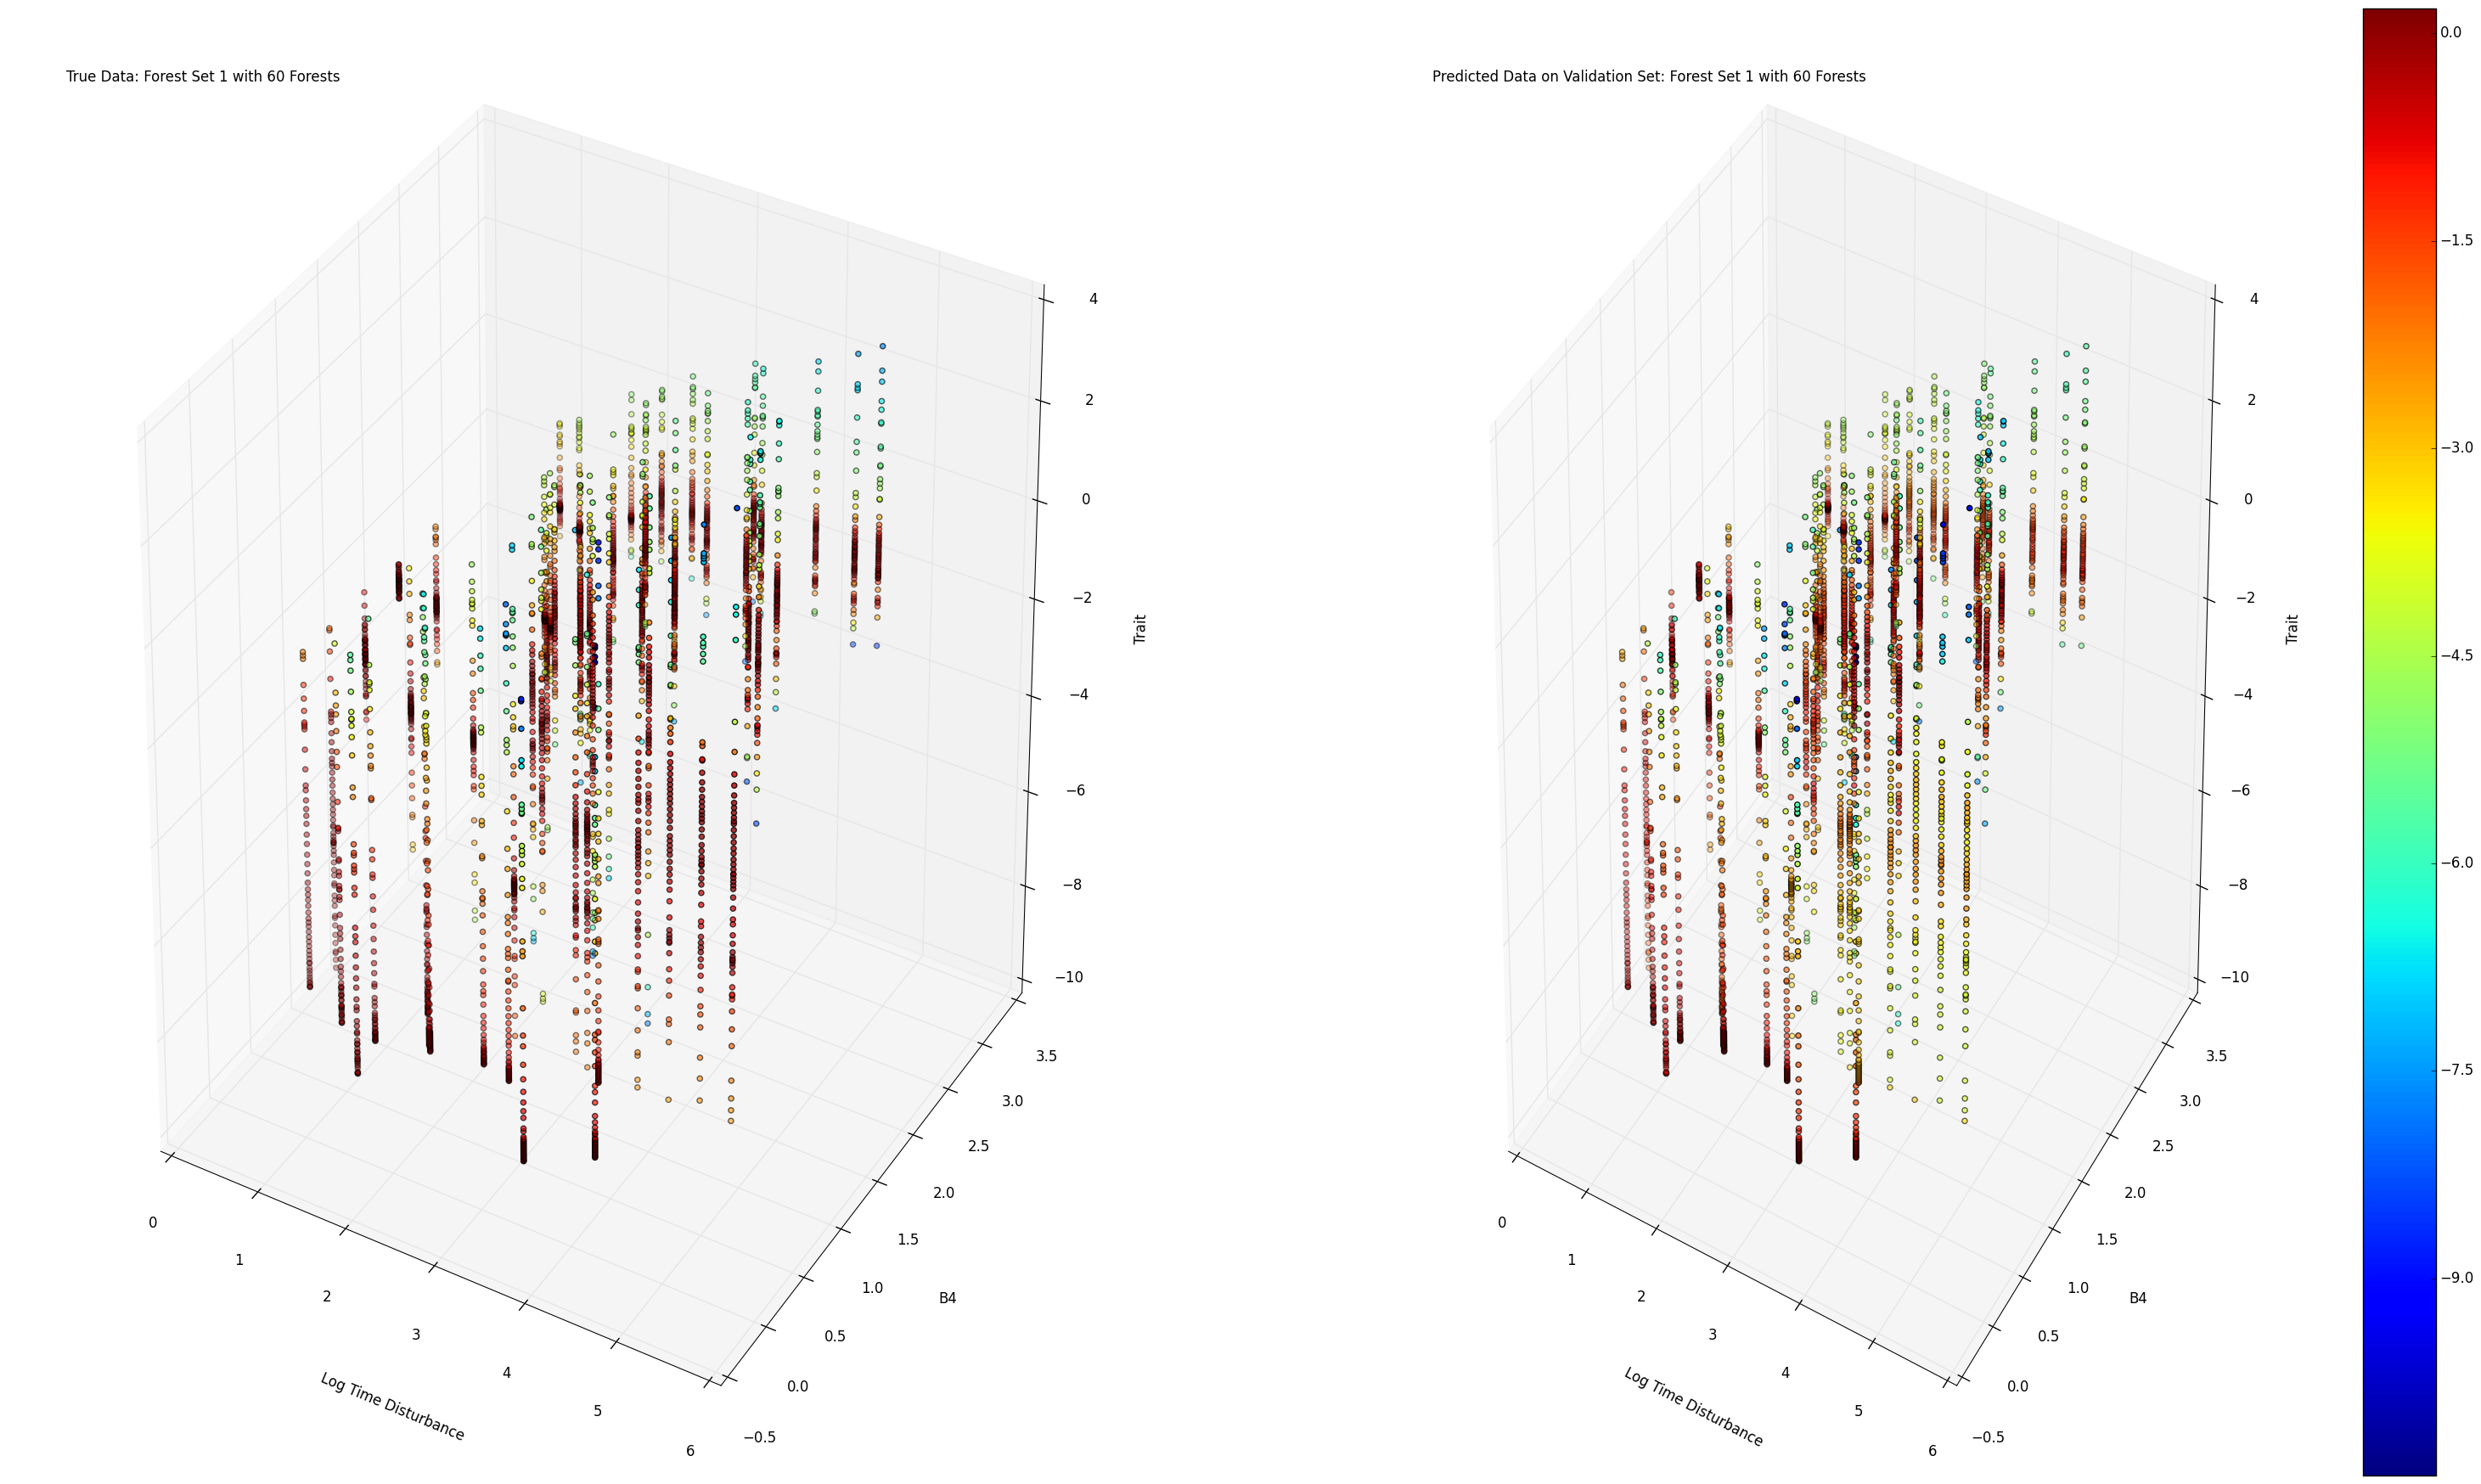
\includegraphics[width=0.9\textwidth]{Figures/Progress/gpr_3D.png}
					\caption{Gaussian Process Single-Task Regression: 3D Example \\
					Kernel Employed: \matern 3/2 Kernel \\
					Left: Training \qquad \qquad \qquad \qquad \qquad Right: Validation}
					\label{ProgressReport:GaussianProcessModels:Figure:gpr_3D}
				\end{figure}
				
				\FloatBarrier
				
				As it is difficult to assess the validation performance from \cref{ProgressReport:GaussianProcessModels:Figure:gpr_3D}, each vertical strand of data is visualised in 1D. Figure \ref{ProgressReport:GaussianProcessModels:Figure:gpr_train} shows 9 strands of data used for training, while \cref{ProgressReport:GaussianProcessModels:Figure:gpr_valid} shows 9 strands of data used for validation. These figures show that the prediction for training data is accurate (evidenced by prediction mean) and precise (evidenced by predicted variance). Similarly, the prediction for validation data is accurate yet less precise, as expected as these were not part of the training set.
				
				\begin{figure}[!htbp]
					\centering
						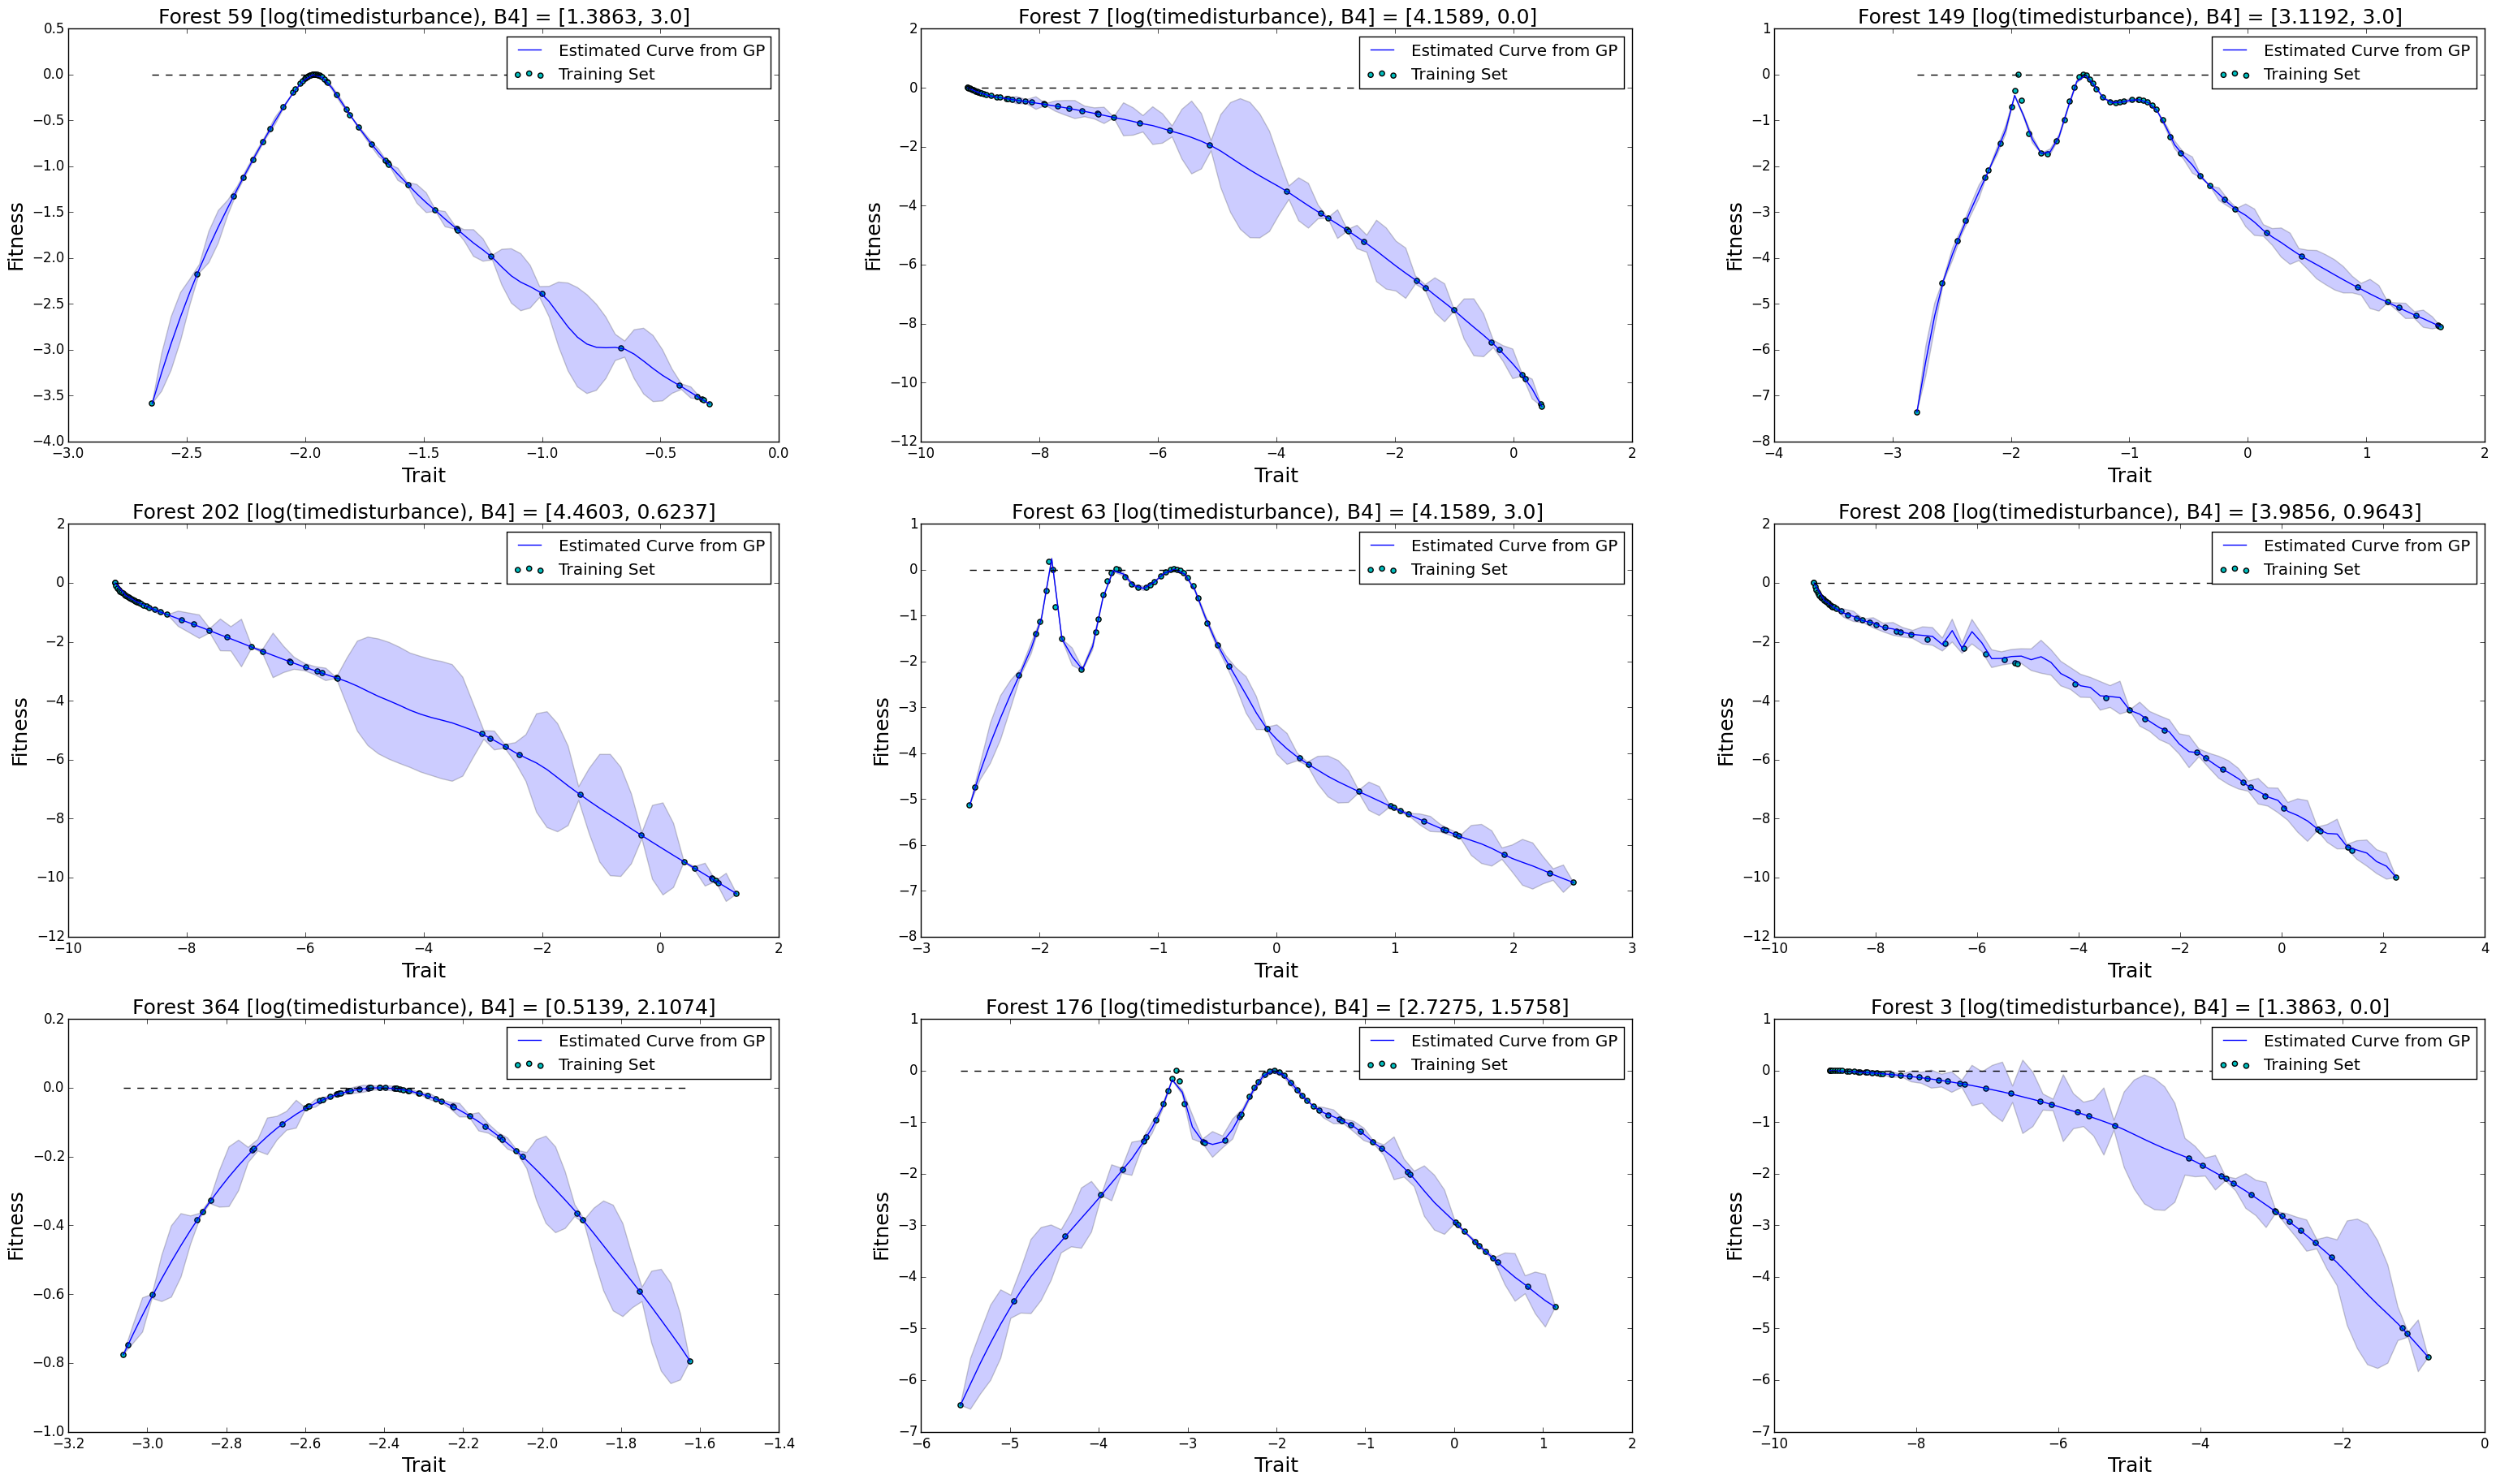
\includegraphics[width=0.9\textwidth]{Figures/Progress/gpr_train.png}
					\caption{GP Single-Task Regression: 3D Example Projected - Training}
					\label{ProgressReport:GaussianProcessModels:Figure:gpr_train}
				\end{figure}

				\begin{figure}[!htbp]
					\centering
						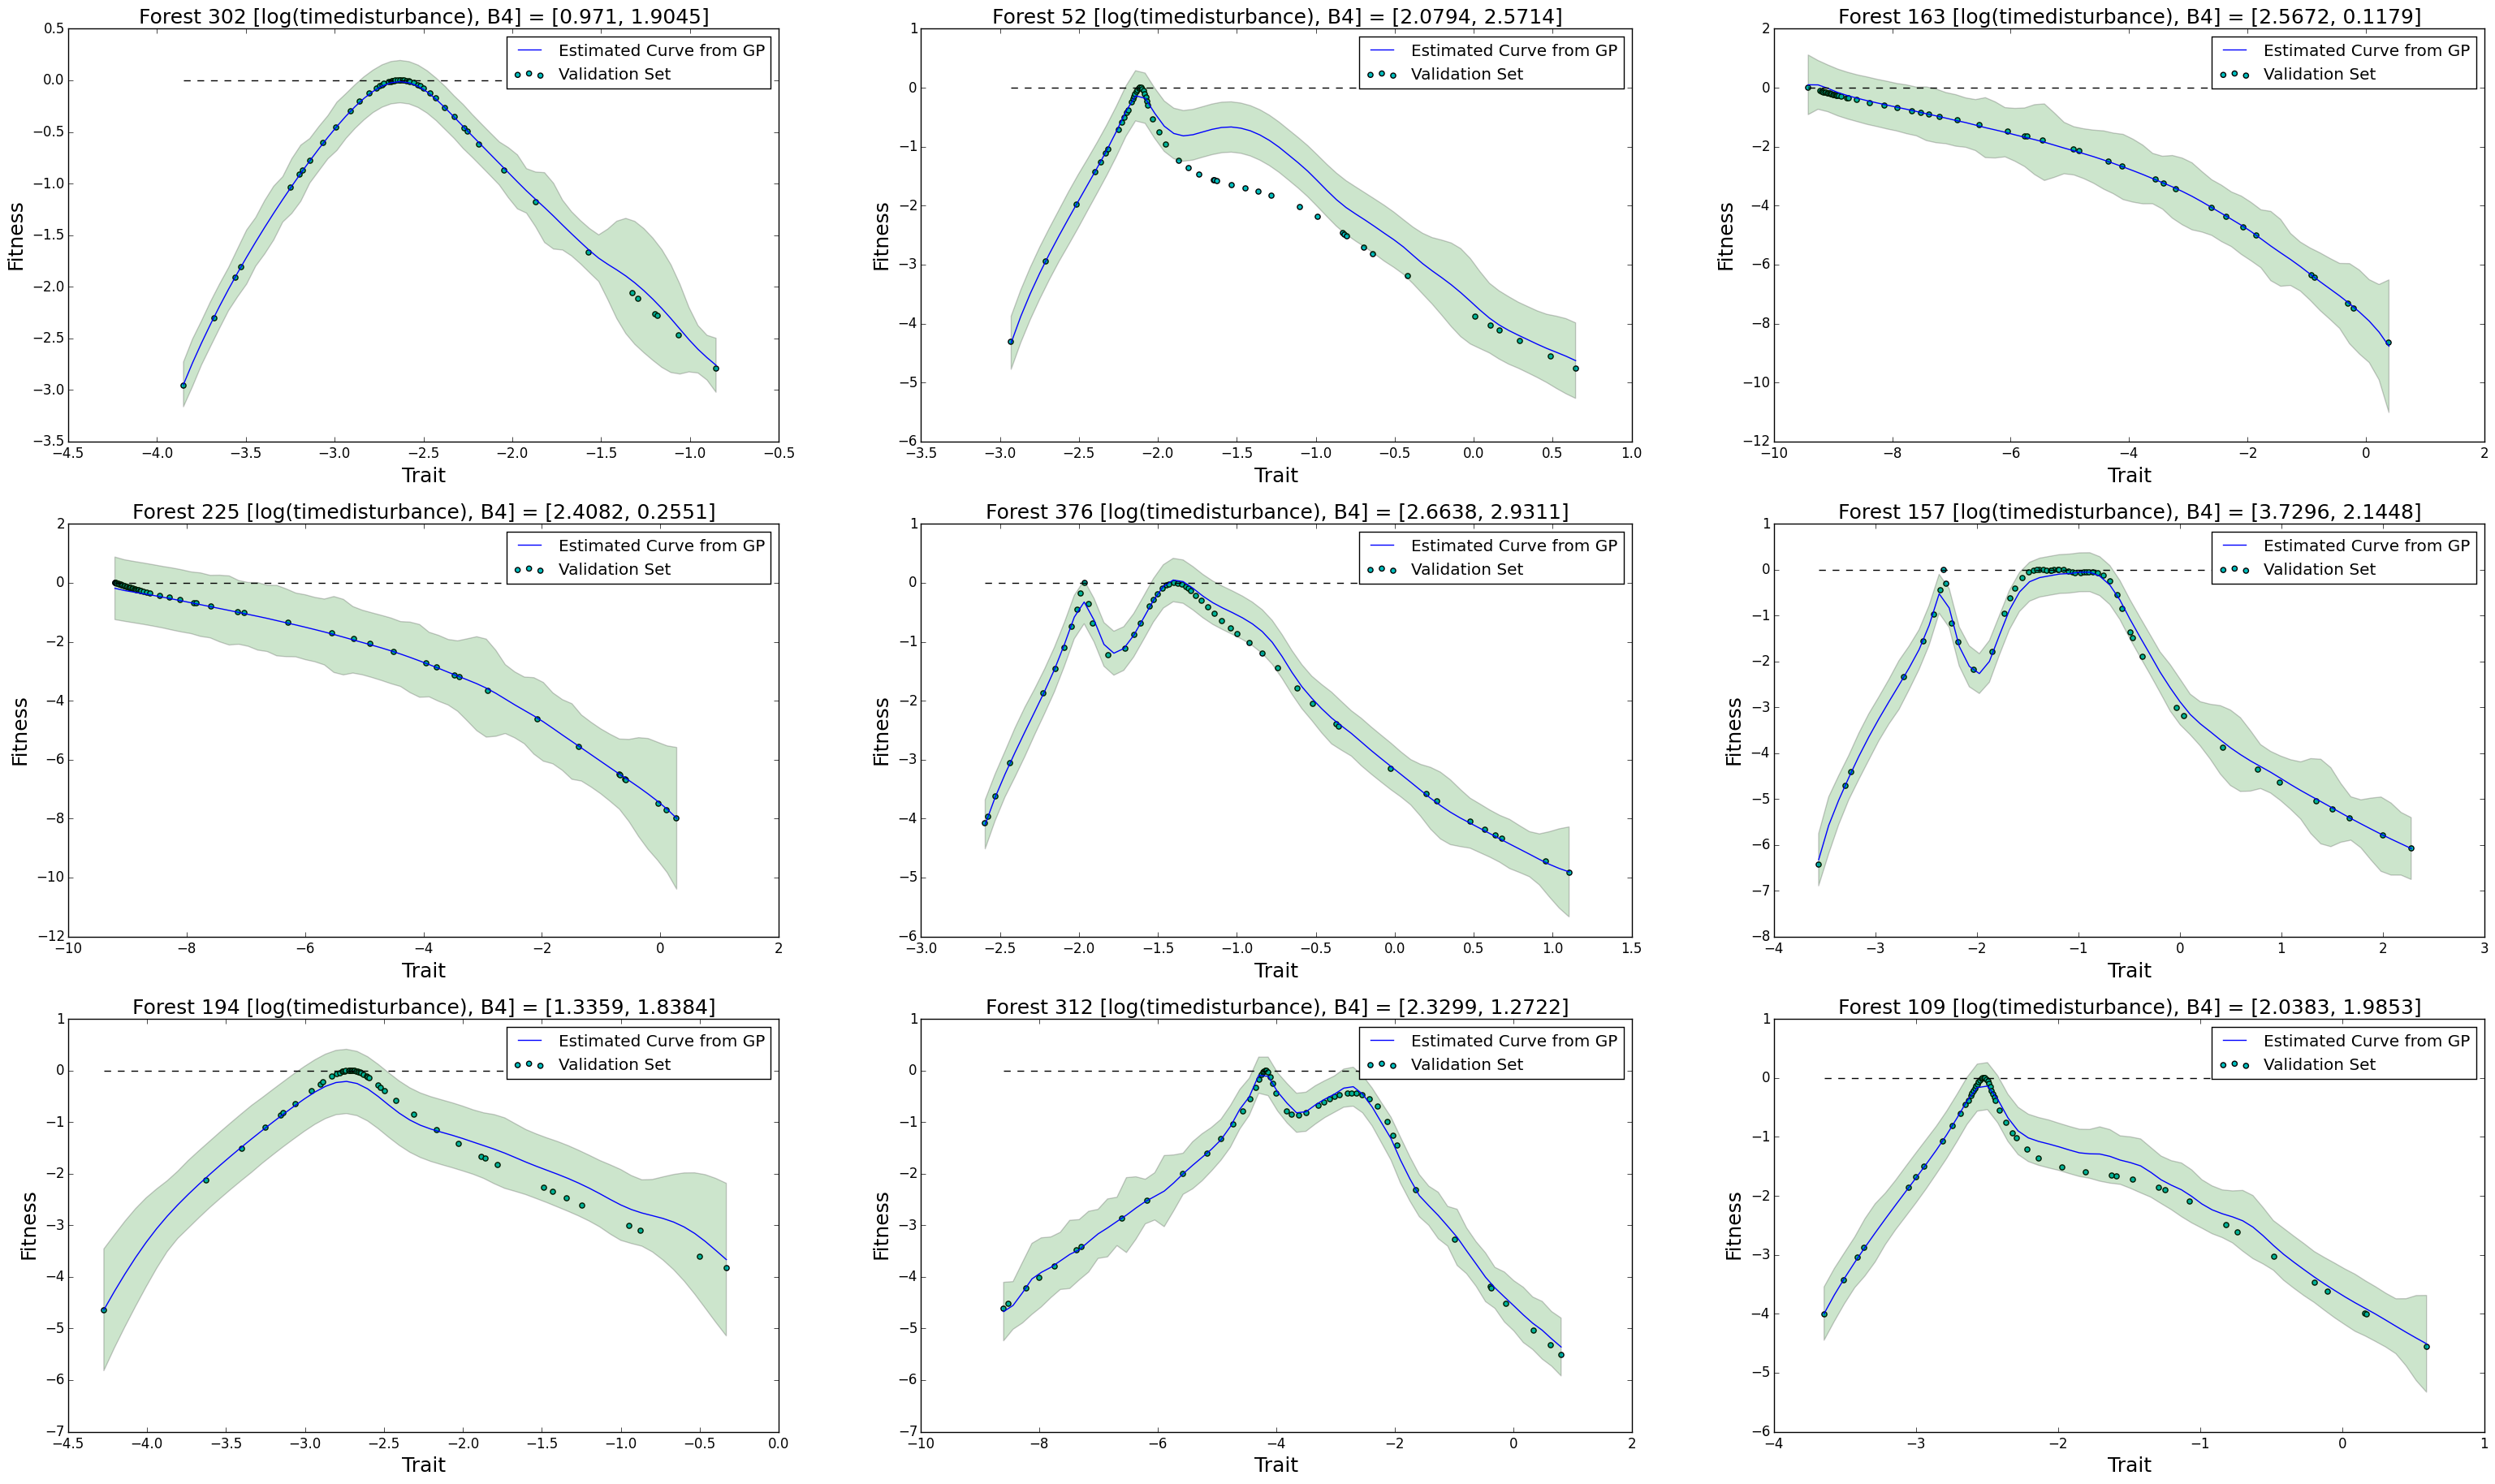
\includegraphics[width=0.9\textwidth]{Figures/Progress/gpr_valid.png}
					\caption{GP Single-Task Regression: 3D Example Projected - Validation}
					\label{ProgressReport:GaussianProcessModels:Figure:gpr_valid}
				\end{figure}
						
				These examples also serve to show a subtle problem with the use of stationary kernels. With attention in \cref{ProgressReport:GaussianProcessModels:Figure:gpr_train}, it is evident that the length scale is too small at certain places, which leads to large uncertainty in regions without data, even though they lie between regions with data exhibiting clear patterns. This is especially the case for the data strand in row 2 column 1 of \cref{ProgressReport:GaussianProcessModels:Figure:gpr_train}, where the GP model is unable to conclude that the pattern is monotonically decreasing in the middle while it is quite evident it should be so from neighboring data.
				
				The reason of this behaviour is that the kernel employed is an axis-aligned stationary kernel. This means that within each axis, the length scale of the kernel is fixed. However, this is a relatively large data set, so there are places where quick variations occur, such as row 2 column 2 of \cref{ProgressReport:GaussianProcessModels:Figure:gpr_train} showing multiple short scale peaks. As a result, the entire length scale in this axis is shortened to model those short scale peaks. As a side consequence, places with scarce data also have short length scales, leading to fast decaying correlation as distance from data points increase and thus increasing the uncertainty in those regions unnecessarily.
				
				This is indeed a problem for exploration. These regions of unnecessarily high uncertainty will increase the entropy of that area even though there exists no interesting properties to be discovered. It is desired that the model only predicts with high entropy at places that it actually cannot model well or know about. For this reason, non-stationary kernels are implemented and discussed in \cref{ProgressReport:GaussianProcessModels:NonStationaryKernels}.
								
				\FloatBarrier
						
			\subsubsection{Multi-task Regression}

				Multi-task regression is useful in bathymetric modeling as it can fill in data when the data is available in different quantities. For example, one data set records depth while the other records pressure, and are recorded at different feature inputs. While the pressure can be modeled as a feature to predict the depth output, it can be more straightforward to perform two GP regression models on the same set of features (a simple one being just the northings-eastings location, which would make this equivalent to a terrain modeling problem). The multi-task regression model can then learn the relationship between the outputs instead of treating them as separate problems. In this way, the depth GP model can do better than resorting to the prior at places without depth data if there exists pressure data at those places.
				
				A simple illustration is presented in \cref{ProgressReport:GaussianProcessModels:Figure:multitask}. The data sets belong to the two tasks partially overlap in the feature space. At places with no overlap, however, the tasks help each other by extrapolating the pattern at places with overlap. In this example, the GP model learned that the two signals are out of phase with each other. Without multi-tasking, the two tasks would return to the prior function (the zero function) quickly at regions without data.
				
				\begin{figure}[!htbp]
					\centering
						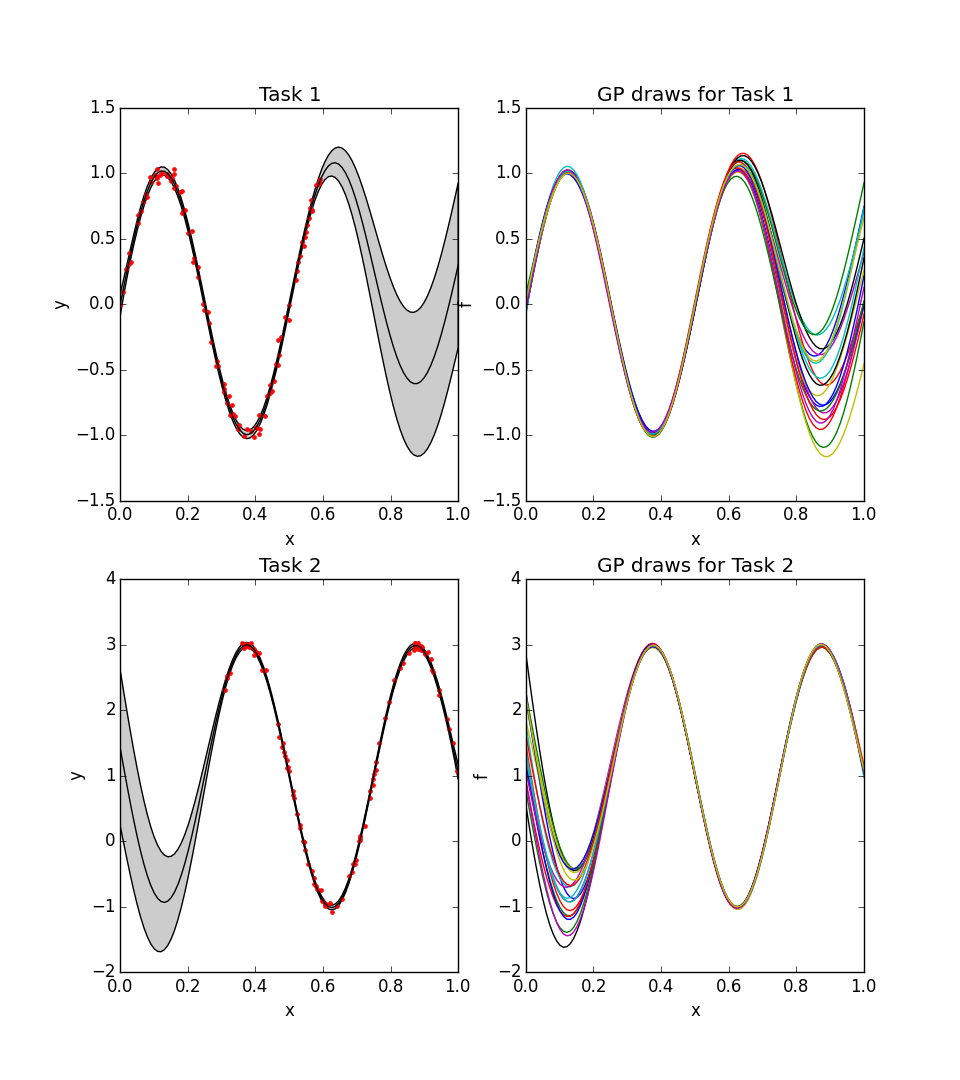
\includegraphics[width=0.9\textwidth]{Figures/Progress/multitask.png}
					\caption{Gaussian Process Multi-Task Regression}
					\label{ProgressReport:GaussianProcessModels:Figure:multitask}
				\end{figure}
							
				\FloatBarrier
			
		\subsection{Classification}
		
			The most important class of models needed for environment modeling is the GP classification model (see \cref{Background:OceanEnvironmentModeling}). This section presents some sample results and figures as generated from the GP libraries that have been built.
			
			Unlike the regression case, because the output labels are no longer continuous, it cannot be represented by a continuous probability density function such as a Gaussian. As outlined in \cref{Background:GaussianProcesses:Classification}, GP classification is done through learning a latent function which is continuous that in turn represents the likelihood of each label under a sigmoid transformation. The final posterior probability, however, is still non-Gaussian. There exists four methods to mitigate this problem. In coherence with \cref{Background:GaussianProcesses:Classification}, the Laplace approximation method is employed.
			
			In the following section, subplot $(i, j)$ of a figure refers to the subplot located at row $i$ and column $j$ of the said figure.
						
			\subsubsection{Binary Classification}

				Binary classification involves categorising labels into two classes. Figure \ref{ProgressReport:GaussianProcessModels:Figure:binary} shows a sample result for binary classification using the Laplace approximation. The figures show the training labels, prediction probabilities, prediction, and prediction entropy respectively.
				
				From here on, all prediction probability plots (subplot (1, 2) for example) are drawn with a level set at $p = 0.5$, unless otherwise stated. This $p = 0.5$ prediction probability boundary are used to obtain the final prediction class in the binary case (subplot (2, 1)). The prediction entropy plots (subplot (2, 2) for example) are drawn with a level set at its $90^{\mathrm{th}}$ quantile, such that the enclosed region, if any, are regions of highest entropy.
				
				\begin{figure}[!htbp]
					\centering
						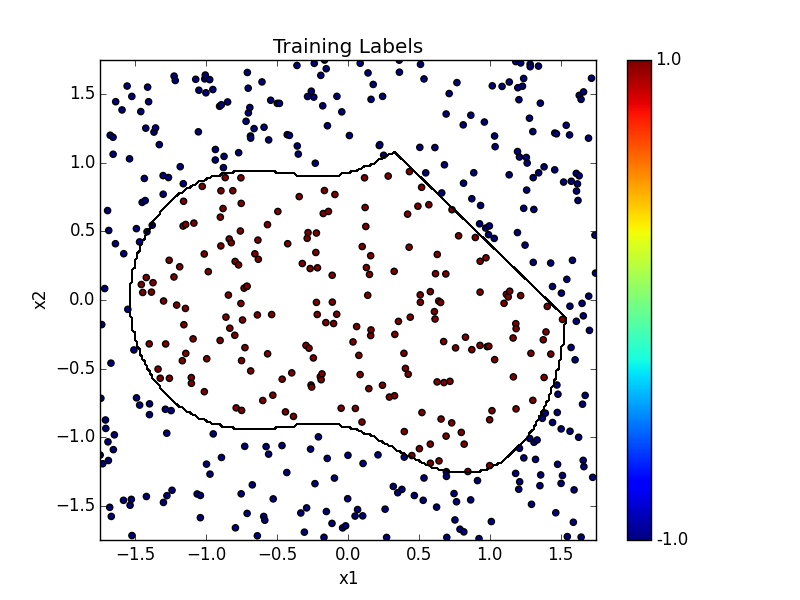
\includegraphics[width=0.48\textwidth]{Figures/Progress/binary/Figure1.png}
						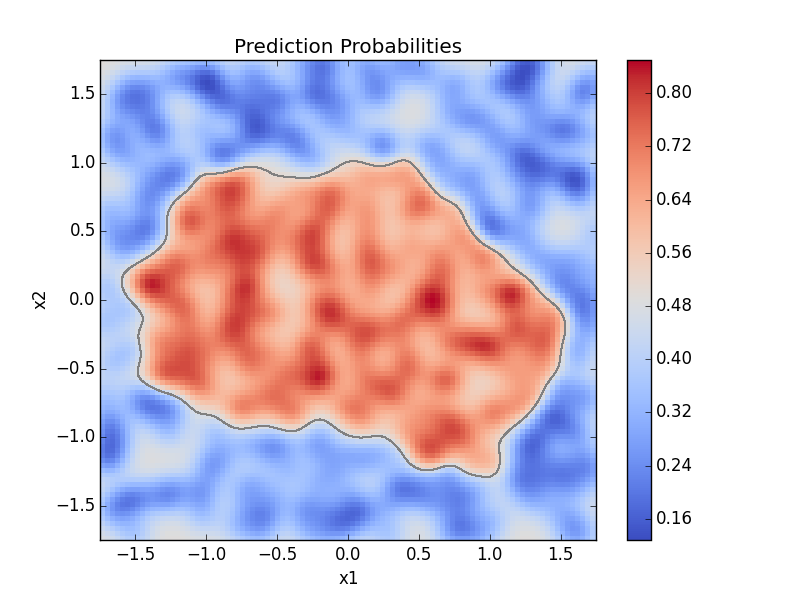
\includegraphics[width=0.48\textwidth]{Figures/Progress/binary/Figure2.png}
						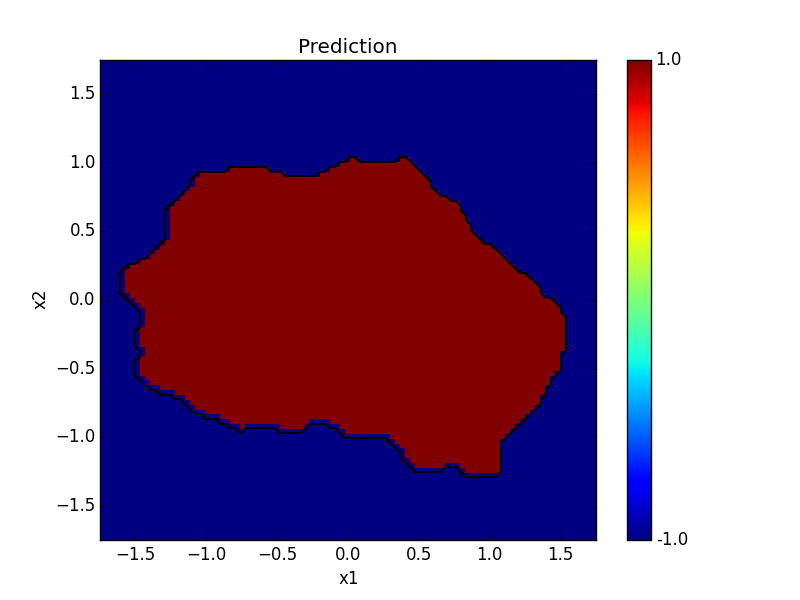
\includegraphics[width=0.48\textwidth]{Figures/Progress/binary/Figure3.png}
						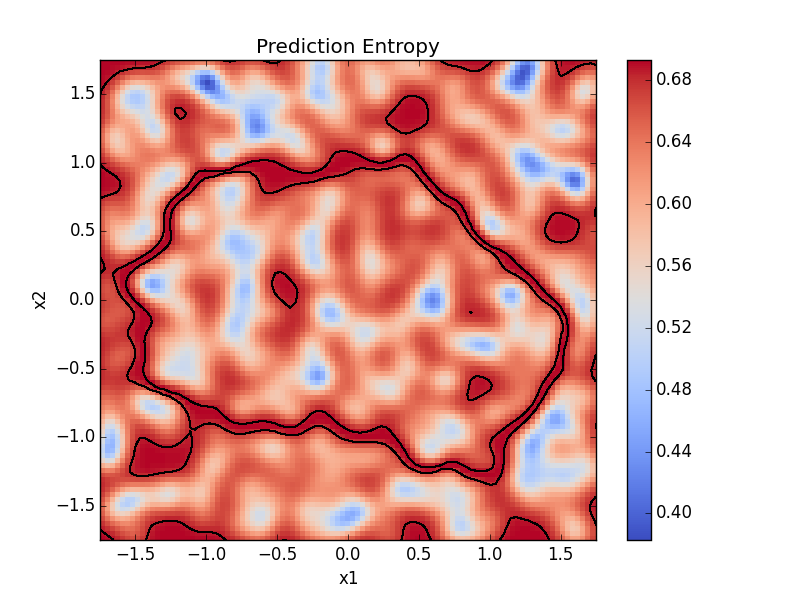
\includegraphics[width=0.48\textwidth]{Figures/Progress/binary/Figure4.png}
					\caption{Gaussian Process Binary Classification}
					\label{ProgressReport:GaussianProcessModels:Figure:binary}
				\end{figure}
							
				This result shows that the prediction is fairly accurate from visual inspection. Most importantly, the places with highest entropy is exact where it is intended to be - at the boundary between the two labels. In fact, a closer examination reveals that the entropy is also high at places without data. Both characteristics are useful for ocean exploration, in order to select the most interesting places where the model cannot decide between labels, and the places with the least amount of information. In fact, the former is often of more interest to the mission. In order to reduce the entropy at places where data is lacking but not near any missing boundaries, the non-stationary kernel function is again used. This will ensure that regions with uniform labels have large length scales, while the boundaries will result in short length scales. As presented lated in \cref{ProgressReport:GaussianProcessModels:NonStationaryKernels}, in this way both the entropy and length scale will accurately pinpoint interesting places with conflicting labels for exploration.
				
				\FloatBarrier
											
			\subsubsection{Multi-class Classification: One v.s. All}
			
				While there is a coherent method for multi-class classification using the Laplace approximation, a simpler approach in which many multi-class classifiers employ is to perform several sets of binary classification and fuse the final result together in a coherent way. The probability fusion is necessary since each binary classifier operates separately without knowledge of each other, and may thus produce conflicting results.
				
				There are two major schemes for which this can be achieved - One v.s. All (OVA) and All v.s. All (AVA), both of which whose background is covered in \cref{Background:GaussianProcesses:Classification}. 
				
				This section and the next presents the test results for the implemented OVA and AVA scheme respectively using the GP binary classifier. Throughout the two sections, the same training set is used, so that comparisons are more direct and consistent.
				
				There are many ways to fuse the final prediction class probability distribution together into a coherent prediction distribution. In this thesis, two methods have been investigated and implemented. At the current stage, the names given to these methods are the \textit{exclusion method} and the \textit{mode keeping method}. These methods are developed and presented in \cref{Background:GaussianProcesses:Classification}. 
				
				\textbf{Exclusion Method}
				
				Figure \ref{ProgressReport:GaussianProcessModels:Figure:exclusionOVA1}, \ref{ProgressReport:GaussianProcessModels:Figure:exclusionOVA2}, and \ref{ProgressReport:GaussianProcessModels:Figure:exclusionOVA3} show the results with the exclusion method. Below are some summary remarks regarding the figures.
				
				\begin{itemize}
					\item The prediction (subplot (2, 2) of \cref{ProgressReport:GaussianProcessModels:Figure:exclusionOVA1}) closely resembles the true situation.
					\item The prediction entropy (subplot (1, 2) and (2, 1) of \cref{ProgressReport:GaussianProcessModels:Figure:exclusionOVA1}) successfully picks out decision boundaries, but only at certain places.
					\item The final fused prediction probabilities (\cref{ProgressReport:GaussianProcessModels:Figure:exclusionOVA2}) and the raw binary prediction probabilities (\cref{ProgressReport:GaussianProcessModels:Figure:exclusionOVA3}) from the binary classifiers are almost identical, although small differences can be seen. 
				\end{itemize}
				
				\begin{figure}[!htbp]
					\centering
						\includegraphics[width=0.48\textwidth]{Figures/Progress/exclusionOVA/Figure1.png}
						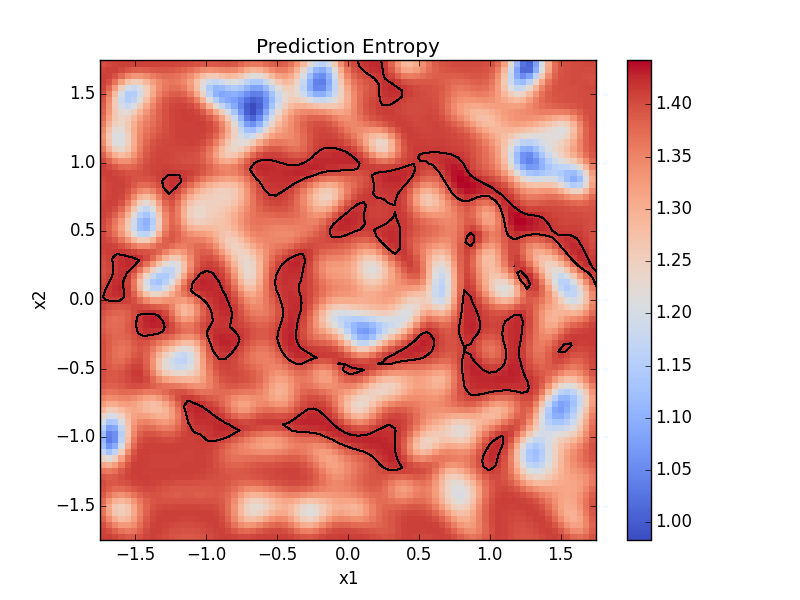
\includegraphics[width=0.48\textwidth]{Figures/Progress/exclusionOVA/Figure2.png}
						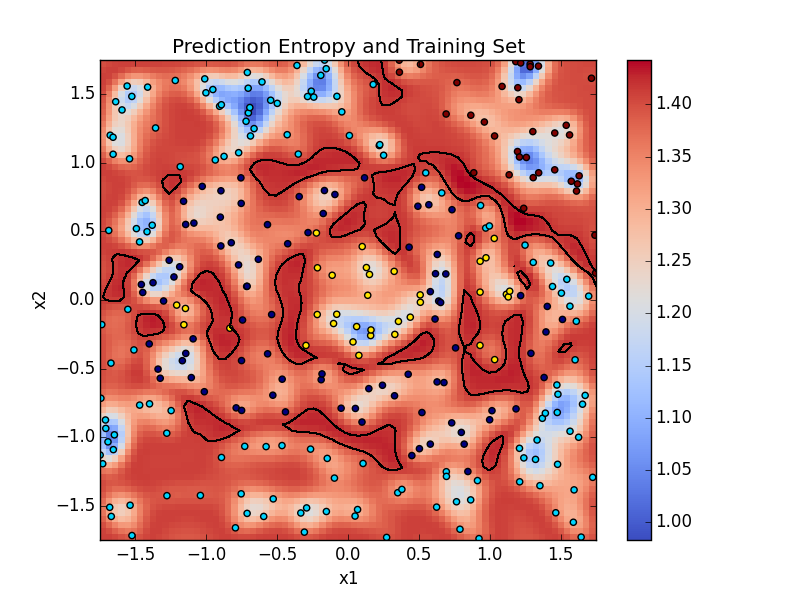
\includegraphics[width=0.48\textwidth]{Figures/Progress/exclusionOVA/Figure3.png}
						\includegraphics[width=0.48\textwidth]{Figures/Progress/exclusionOVA/Figure4.png}
					\caption{GP Multi-Class One v.s. All Classification using Exclusion Method}
					\label{ProgressReport:GaussianProcessModels:Figure:exclusionOVA1}
				\end{figure}

				\begin{figure}[!htbp]
					\centering
						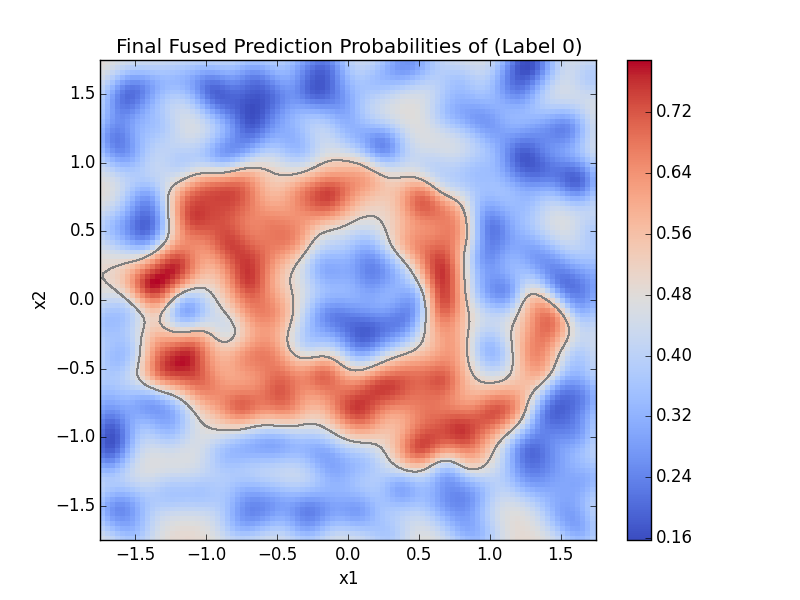
\includegraphics[width=0.48\textwidth]{Figures/Progress/exclusionOVA/Figure5.png}
						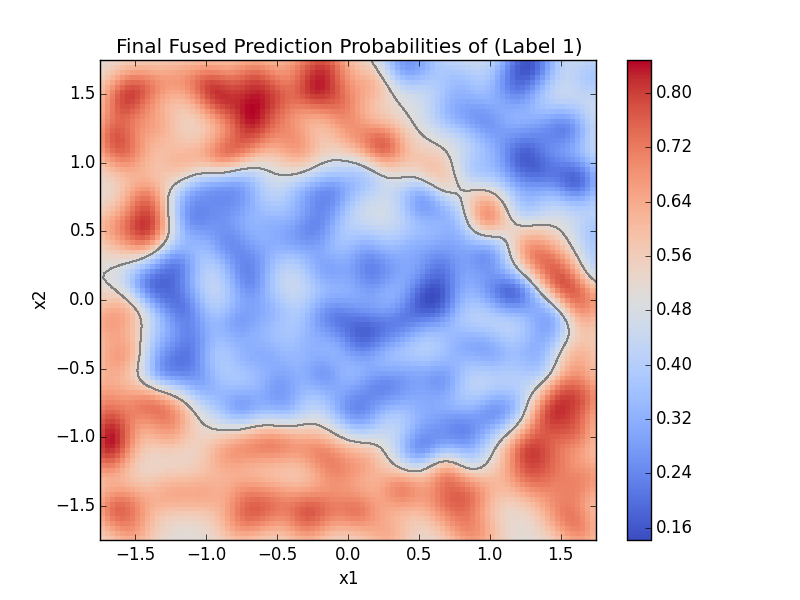
\includegraphics[width=0.48\textwidth]{Figures/Progress/exclusionOVA/Figure6.png}
						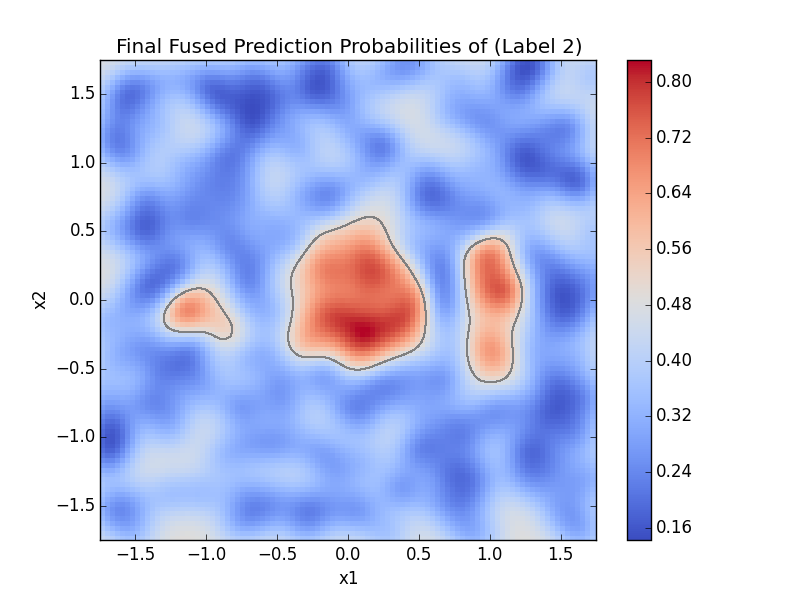
\includegraphics[width=0.48\textwidth]{Figures/Progress/exclusionOVA/Figure7.png}
						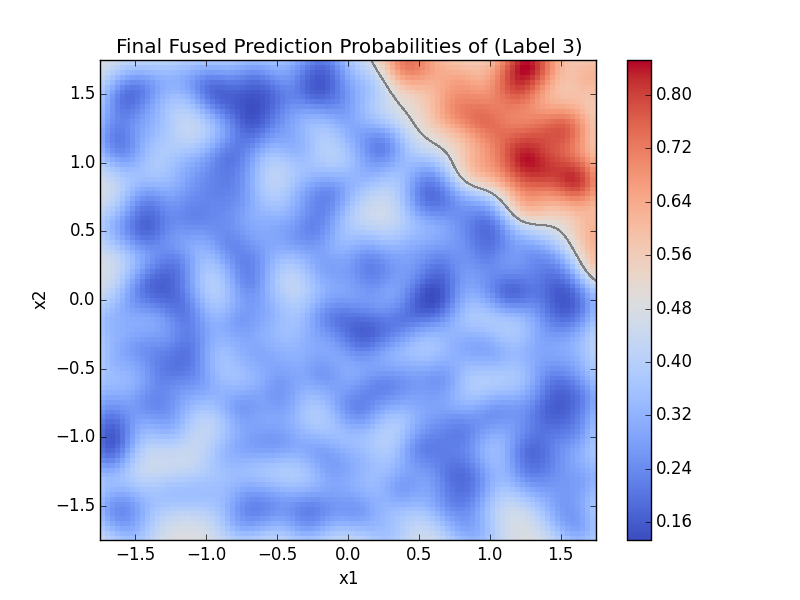
\includegraphics[width=0.48\textwidth]{Figures/Progress/exclusionOVA/Figure8.png}
					\caption{GP Multi-Class One v.s. All Classification using Exclusion Method}
					\label{ProgressReport:GaussianProcessModels:Figure:exclusionOVA2}
				\end{figure}
				
				\begin{figure}[!htbp]
					\centering
						\includegraphics[width=0.48\textwidth]{Figures/Progress/exclusionOVA/Figure9.png}
						\includegraphics[width=0.48\textwidth]{Figures/Progress/exclusionOVA/Figure10.png}
						\includegraphics[width=0.48\textwidth]{Figures/Progress/exclusionOVA/Figure11.png}
						\includegraphics[width=0.48\textwidth]{Figures/Progress/exclusionOVA/Figure12.png}
					\caption{GP Multi-Class One v.s. All Classification using Exclusion Method}
					\label{ProgressReport:GaussianProcessModels:Figure:exclusionOVA3}
				\end{figure}
				
				\FloatBarrier
				
				\textbf{Mode Keeping Method}
				
				Figure \ref{ProgressReport:GaussianProcessModels:Figure:modekeepingOVA1}, \ref{ProgressReport:GaussianProcessModels:Figure:modekeepingOVA2}, and \ref{ProgressReport:GaussianProcessModels:Figure:modekeepingOVA3} show the results with the mode keeping method. Below are some summary remarks regarding the figures.
				
				\begin{itemize}
					\item The prediction (subplot (2, 2) of \cref{ProgressReport:GaussianProcessModels:Figure:modekeepingOVA1}) closely resembles the true situation.
					\item The prediction entropy (subplot (1, 2) and (2, 1) of \cref{ProgressReport:GaussianProcessModels:Figure:modekeepingOVA1}) successfully picks out decision boundaries very closely and accurately.
					\item The final fused prediction probabilities (\cref{ProgressReport:GaussianProcessModels:Figure:modekeepingOVA2}) and the raw binary prediction probabilities (\cref{ProgressReport:GaussianProcessModels:Figure:modekeepingOVA3}) from the binary classifiers are quite different. While the $p = 0.5$ binary decision boundaries remain similar, the final fused probabilities are more extreme and polar than before. This is expected as the scheme is keeping the mode probability and shifting every other probability down.
					\item This is the best performing scheme in terms of determining the decision boundary.
				\end{itemize}
				
				\begin{figure}[!htbp]
					\centering
						\includegraphics[width=0.48\textwidth]{Figures/Progress/modekeepingOVA/Figure1.png}
						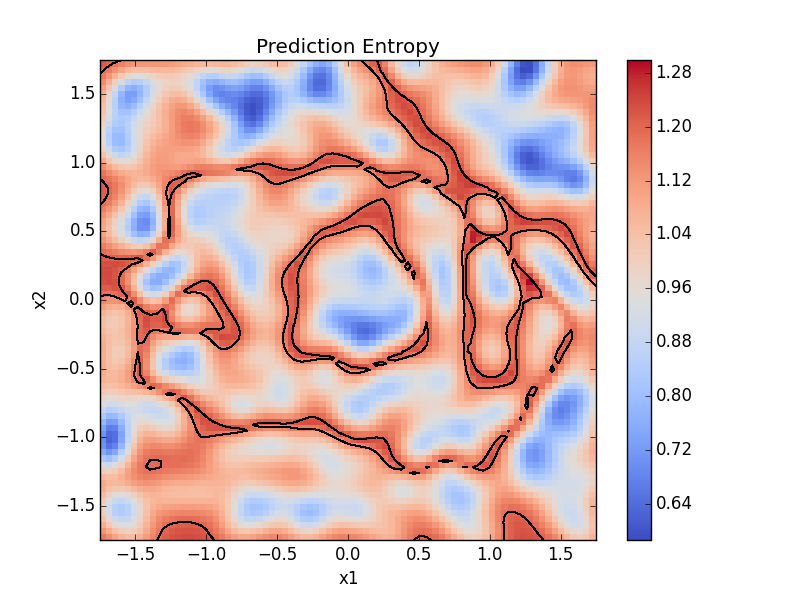
\includegraphics[width=0.48\textwidth]{Figures/Progress/modekeepingOVA/Figure2.png}
						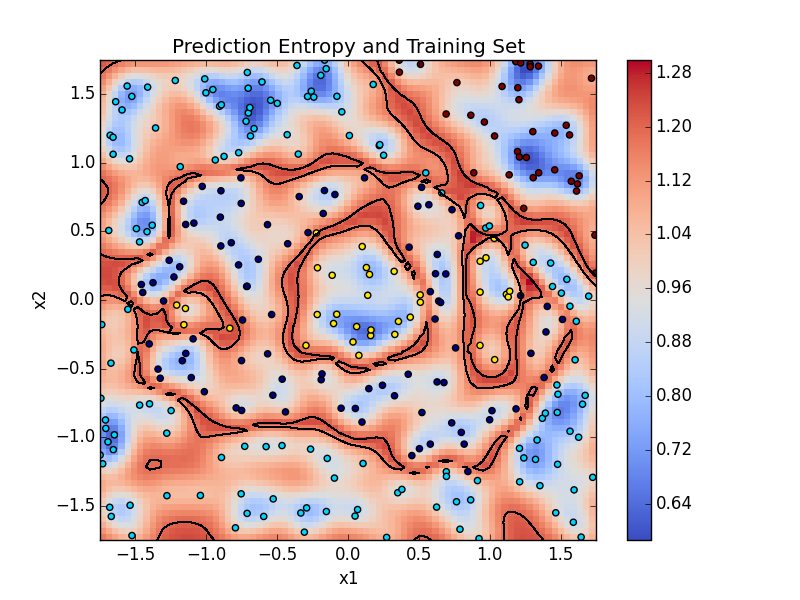
\includegraphics[width=0.48\textwidth]{Figures/Progress/modekeepingOVA/Figure3.png}
						\includegraphics[width=0.48\textwidth]{Figures/Progress/modekeepingOVA/Figure4.png}
					\caption{GP Multi-Class One v.s. All Classification using Mode Keeping Method}
					\label{ProgressReport:GaussianProcessModels:Figure:modekeepingOVA1}
				\end{figure}

				\begin{figure}[!htbp]
					\centering
						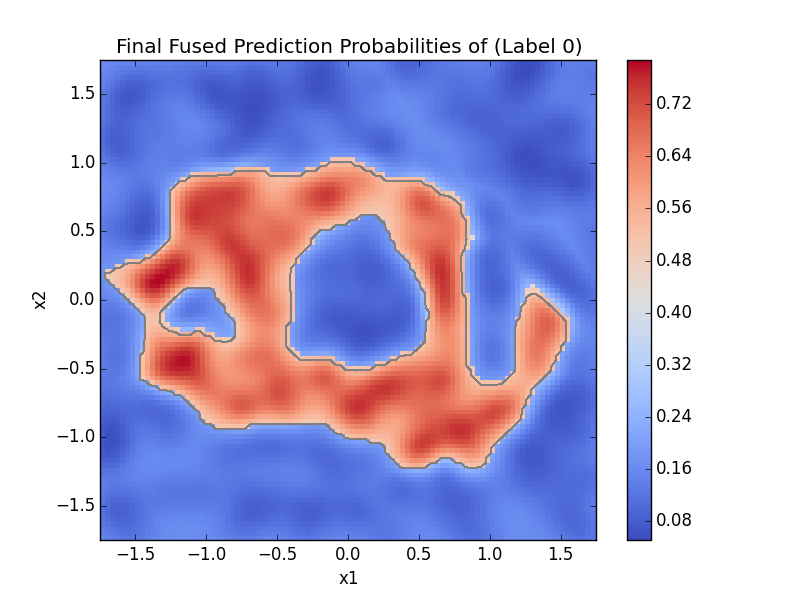
\includegraphics[width=0.48\textwidth]{Figures/Progress/modekeepingOVA/Figure5.png}
						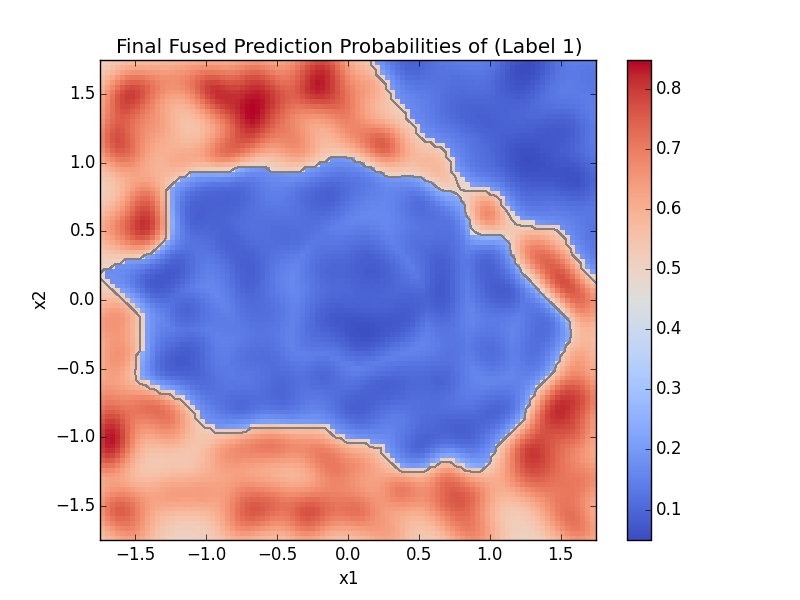
\includegraphics[width=0.48\textwidth]{Figures/Progress/modekeepingOVA/Figure6.png}
						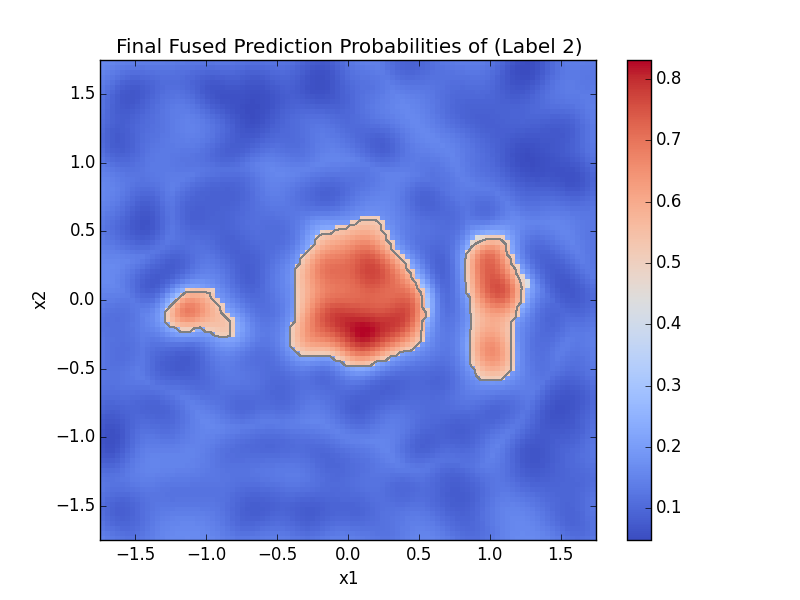
\includegraphics[width=0.48\textwidth]{Figures/Progress/modekeepingOVA/Figure7.png}
						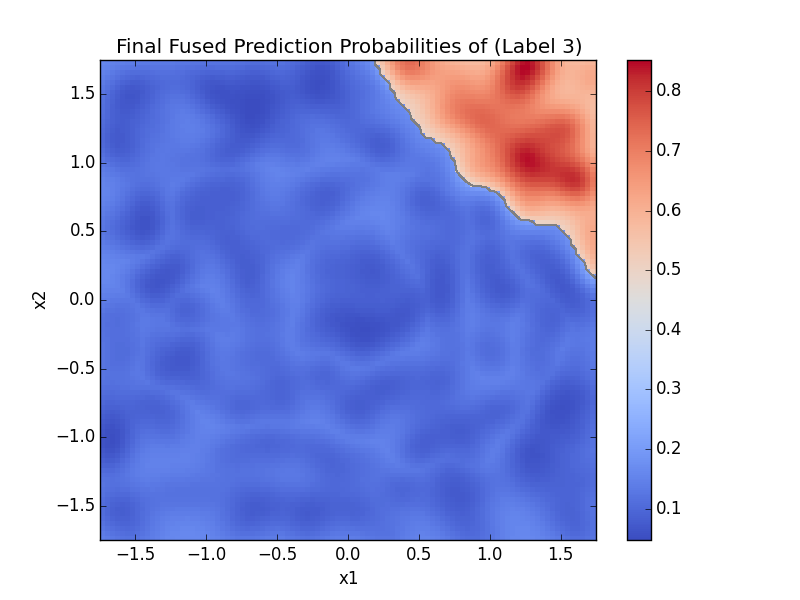
\includegraphics[width=0.48\textwidth]{Figures/Progress/modekeepingOVA/Figure8.png}
					\caption{GP Multi-Class One v.s. All Classification using Mode Keeping Method}
					\label{ProgressReport:GaussianProcessModels:Figure:modekeepingOVA2}
				\end{figure}
				
				\begin{figure}[!htbp]
					\centering
						\includegraphics[width=0.48\textwidth]{Figures/Progress/modekeepingOVA/Figure9.png}
						\includegraphics[width=0.48\textwidth]{Figures/Progress/modekeepingOVA/Figure10.png}
						\includegraphics[width=0.48\textwidth]{Figures/Progress/modekeepingOVA/Figure11.png}
						\includegraphics[width=0.48\textwidth]{Figures/Progress/modekeepingOVA/Figure12.png}
					\caption{GP Multi-Class One v.s. All Classification using Mode Keeping Method}
					\label{ProgressReport:GaussianProcessModels:Figure:modekeepingOVA3}
				\end{figure}
											
				\FloatBarrier
				
			\subsubsection{Multi-class Classification: All v.s. All}

				Figure \ref{ProgressReport:GaussianProcessModels:Figure:exclusionAVA1}, \ref{ProgressReport:GaussianProcessModels:Figure:exclusionAVA2}, and \ref{ProgressReport:GaussianProcessModels:Figure:exclusionAVA3} show the results with the exclusion method. Below are some summary remarks regarding the figures.
				
				\begin{itemize}
					\item The prediction (subplot (2, 2) of \cref{ProgressReport:GaussianProcessModels:Figure:exclusionAVA1}) closely resembles the true situation.
					\item The prediction entropy (subplot (1, 2) and (2, 1) of \cref{ProgressReport:GaussianProcessModels:Figure:exclusionAVA1}) successfully picks out decision boundaries, but only at certain places. This is very similar to the OVA case with the exclusion method. However, it is more evident that this method is tending towards picking places without data as well.
					\item The final fused prediction probabilities (\cref{ProgressReport:GaussianProcessModels:Figure:exclusionAVA2}) and the raw binary prediction probabilities (\cref{ProgressReport:GaussianProcessModels:Figure:exclusionAVA3}) from the binary classifiers are almost identical at the relevant regions. The raw prediction probabilities are close to $p = 0.5$ at irrelevant regions, as expected.
				\end{itemize}
				
				\textbf{Exclusion Method}
				
				\begin{figure}[!htbp]
					\centering
						\includegraphics[width=0.48\textwidth]{Figures/Progress/exclusionAVA/Figure1.png}
						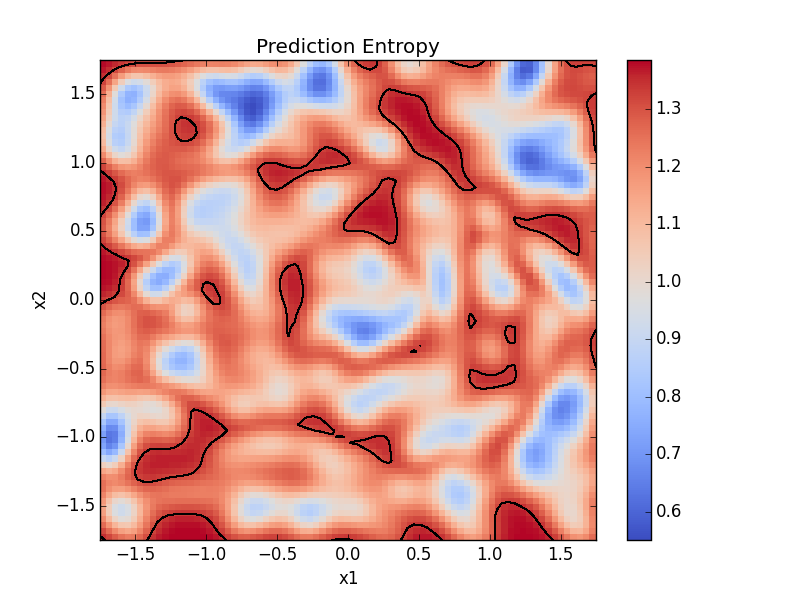
\includegraphics[width=0.48\textwidth]{Figures/Progress/exclusionAVA/Figure2.png}
						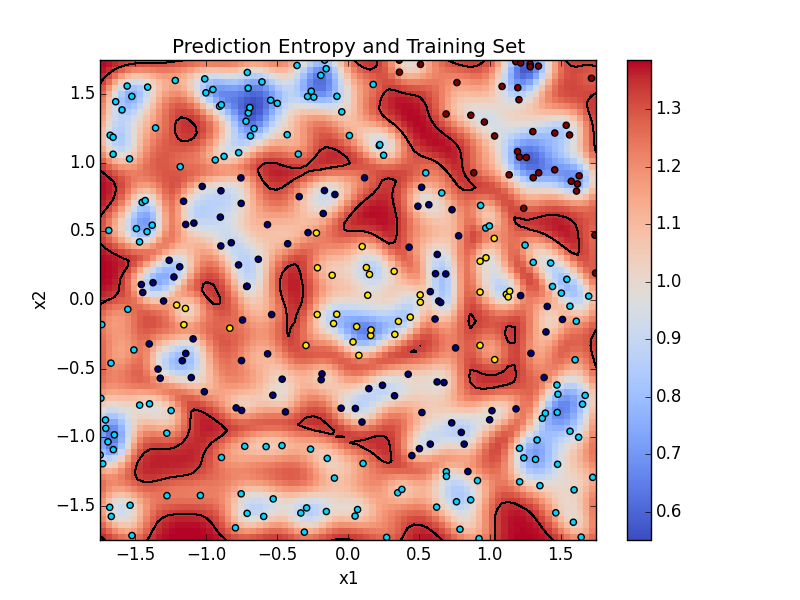
\includegraphics[width=0.48\textwidth]{Figures/Progress/exclusionAVA/Figure3.png}
						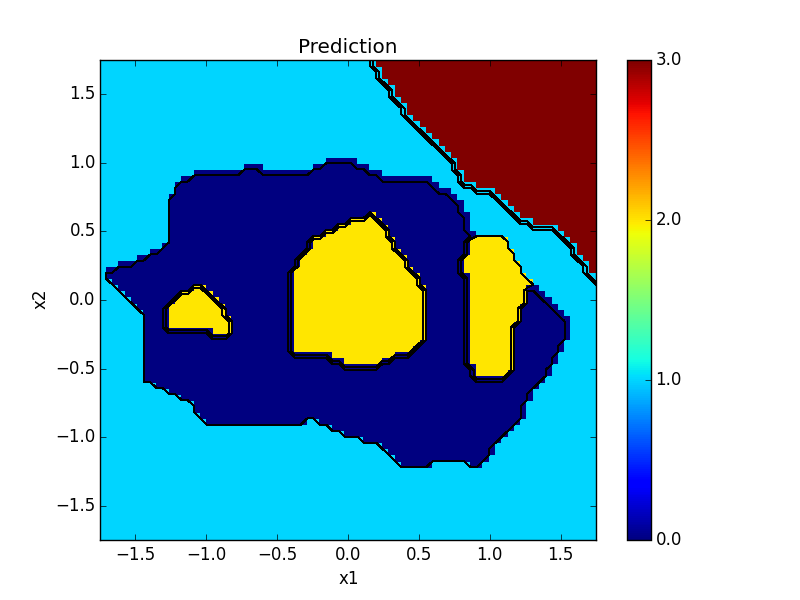
\includegraphics[width=0.48\textwidth]{Figures/Progress/exclusionAVA/Figure4.png}
					\caption{GP Multi-Class All v.s. All Classification using Exclusion Method}
					\label{ProgressReport:GaussianProcessModels:Figure:exclusionAVA1}
				\end{figure}

				\begin{figure}[!htbp]
					\centering
						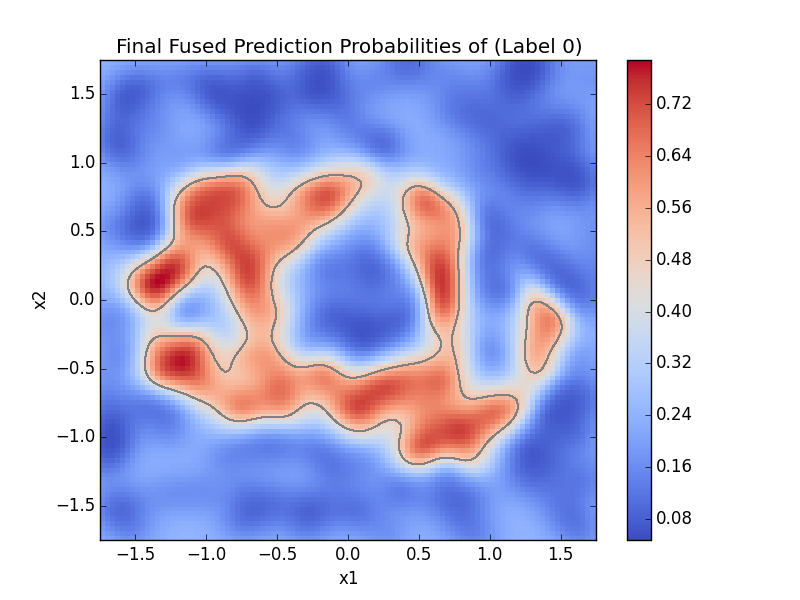
\includegraphics[width=0.48\textwidth]{Figures/Progress/exclusionAVA/Figure5.png}
						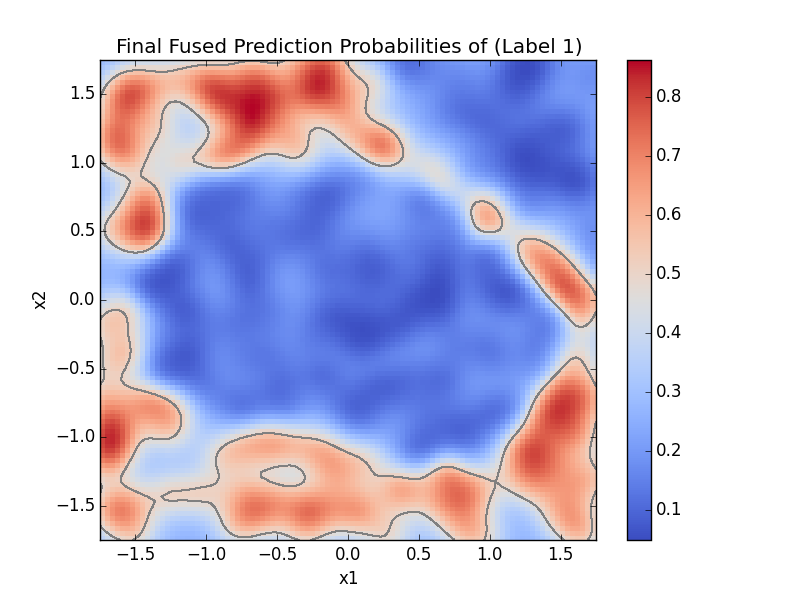
\includegraphics[width=0.48\textwidth]{Figures/Progress/exclusionAVA/Figure6.png}
						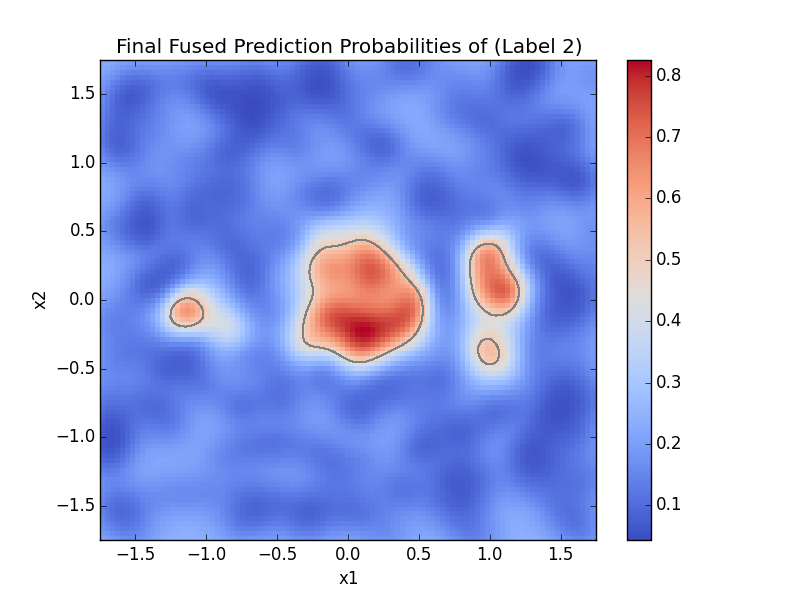
\includegraphics[width=0.48\textwidth]{Figures/Progress/exclusionAVA/Figure7.png}
						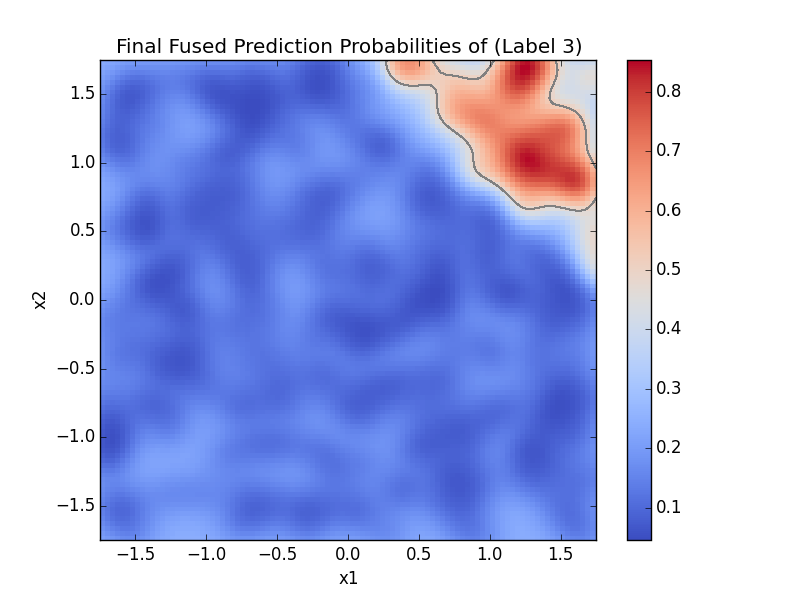
\includegraphics[width=0.48\textwidth]{Figures/Progress/exclusionAVA/Figure8.png}
					\caption{GP Multi-Class All v.s. All Classification using Exclusion Method}
					\label{ProgressReport:GaussianProcessModels:Figure:exclusionAVA2}
				\end{figure}
				
				\begin{figure}[!htbp]
					\centering
						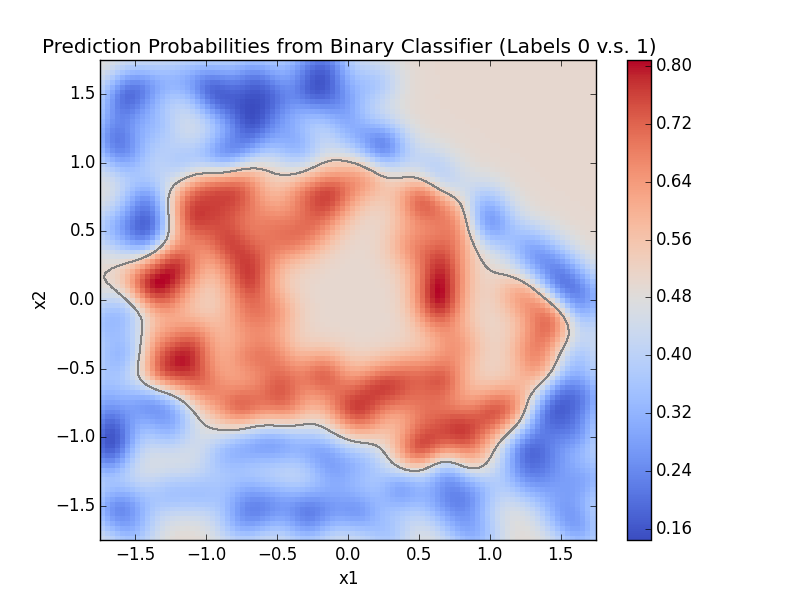
\includegraphics[width=0.48\textwidth]{Figures/Progress/exclusionAVA/Figure9.png}
						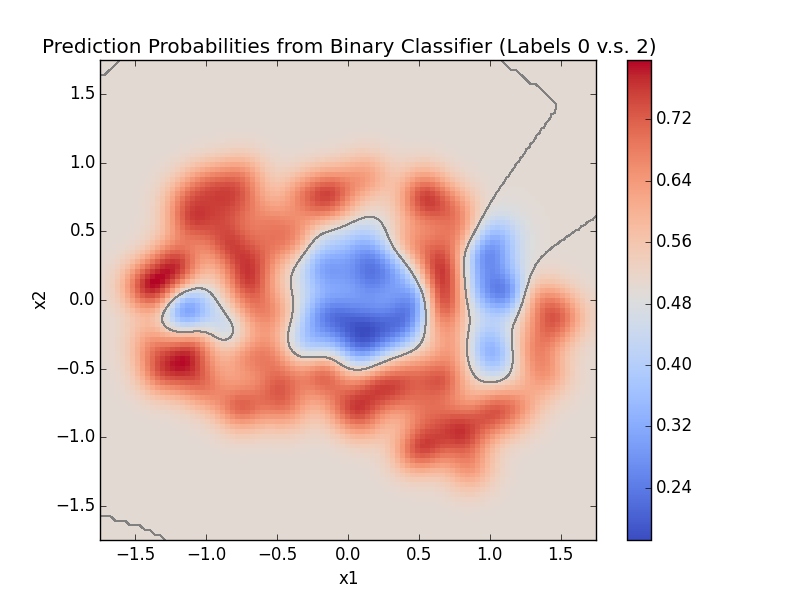
\includegraphics[width=0.48\textwidth]{Figures/Progress/exclusionAVA/Figure10.png}
						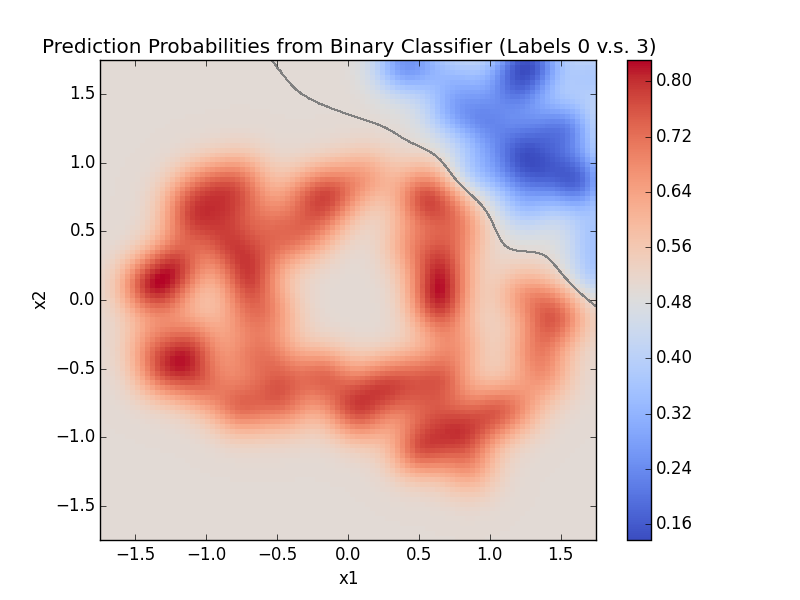
\includegraphics[width=0.48\textwidth]{Figures/Progress/exclusionAVA/Figure11.png}
						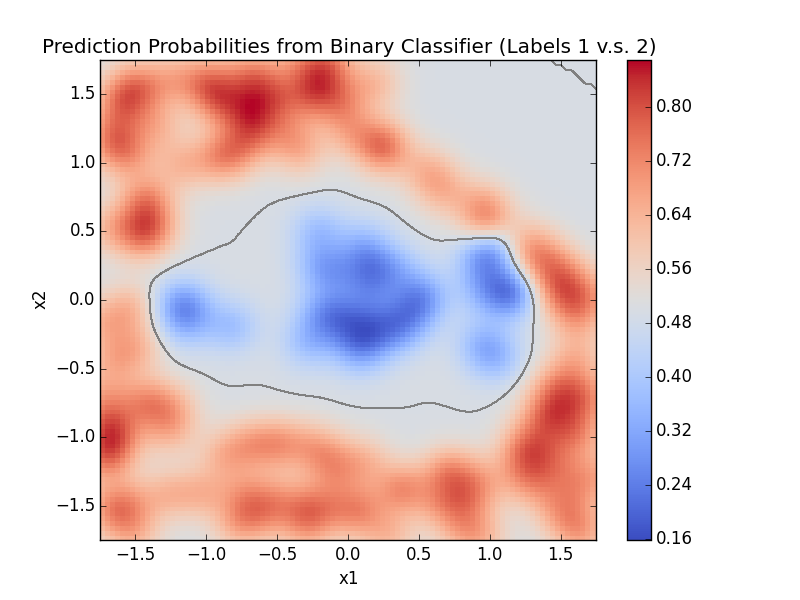
\includegraphics[width=0.48\textwidth]{Figures/Progress/exclusionAVA/Figure12.png}
						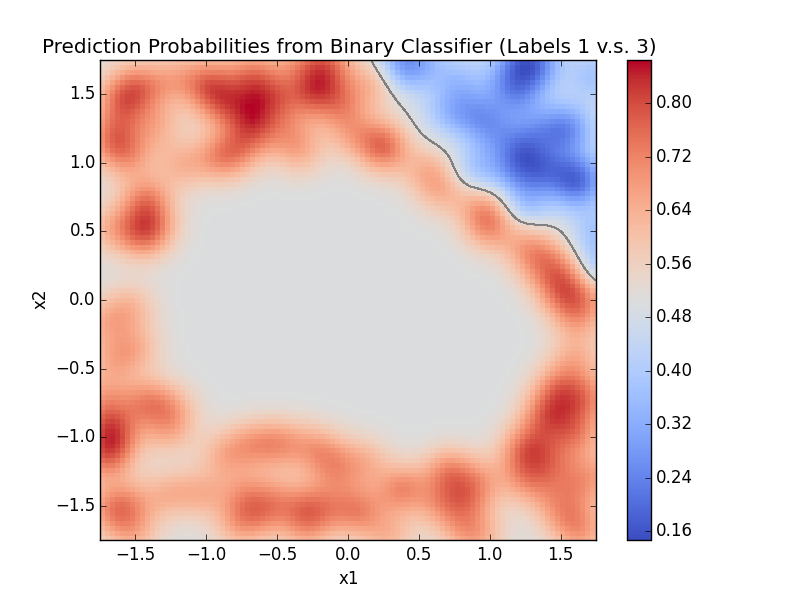
\includegraphics[width=0.48\textwidth]{Figures/Progress/exclusionAVA/Figure13.png}
						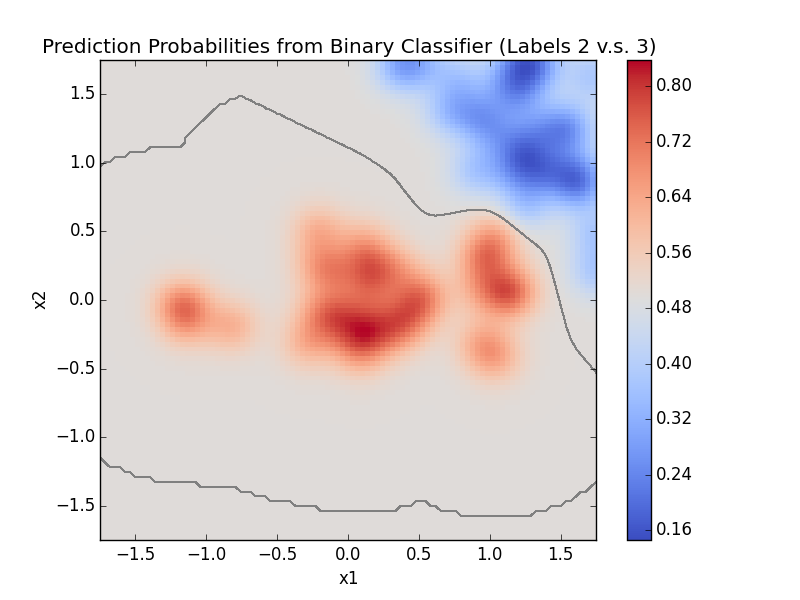
\includegraphics[width=0.48\textwidth]{Figures/Progress/exclusionAVA/Figure14.png}
					\caption{GP Multi-Class All v.s. All Classification using Exclusion Method}
					\label{ProgressReport:GaussianProcessModels:Figure:exclusionAVA3}
				\end{figure}
				
				\FloatBarrier
				
				\textbf{Mode Keeping Method}
				
				Figure \ref{ProgressReport:GaussianProcessModels:Figure:modekeepingAVA1}, \ref{ProgressReport:GaussianProcessModels:Figure:modekeepingAVA2}, and \ref{ProgressReport:GaussianProcessModels:Figure:modekeepingAVA3} show the results with the mode keeping method. Below are some summary remarks regarding the figures.
				
				\begin{itemize}
					\item The prediction (subplot (2, 2) of \cref{ProgressReport:GaussianProcessModels:Figure:modekeepingAVA1}) closely resembles the true situation.
					\item The prediction entropy (subplot (1, 2) and (2, 1) of \cref{ProgressReport:GaussianProcessModels:Figure:modekeepingAVA1}) successfully picks out decision boundaries, however it is not as evident as the OVA case, although arguably on par with the exclusion method.
					\item The final fused prediction probabilities (\cref{ProgressReport:GaussianProcessModels:Figure:modekeepingAVA2}) and the raw binary prediction probabilities (\cref{ProgressReport:GaussianProcessModels:Figure:modekeepingAVA3}) from the binary classifiers are quite different. Similar to the OVA case, while the $p = 0.5$ binary decision boundaries remain similar, the final fused probabilities are more extreme and polar than before.
				\end{itemize}
				\begin{figure}[!htbp]
					\centering
						\includegraphics[width=0.48\textwidth]{Figures/Progress/modekeepingAVA/Figure1.png}
						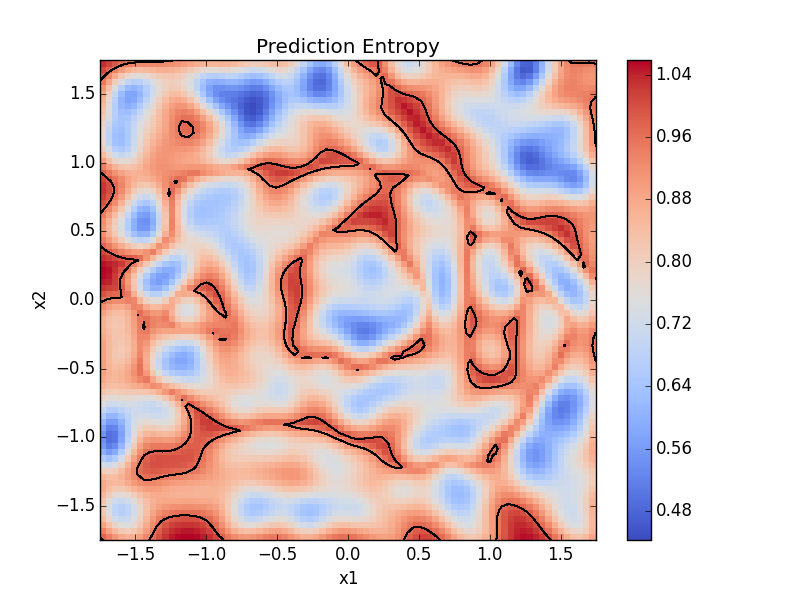
\includegraphics[width=0.48\textwidth]{Figures/Progress/modekeepingAVA/Figure2.png}
						\includegraphics[width=0.48\textwidth]{Figures/Progress/modekeepingAVA/Figure3.png}
						\includegraphics[width=0.48\textwidth]{Figures/Progress/modekeepingAVA/Figure4.png}
					\caption{GP Multi-Class All v.s. All Classification using Mode Keeping Method}
					\label{ProgressReport:GaussianProcessModels:Figure:modekeepingAVA1}
				\end{figure}

				\begin{figure}[!htbp]
					\centering
						\includegraphics[width=0.48\textwidth]{Figures/Progress/modekeepingAVA/Figure5.png}
						\includegraphics[width=0.48\textwidth]{Figures/Progress/modekeepingAVA/Figure6.png}
						\includegraphics[width=0.48\textwidth]{Figures/Progress/modekeepingAVA/Figure7.png}
						\includegraphics[width=0.48\textwidth]{Figures/Progress/modekeepingAVA/Figure8.png}
					\caption{GP Multi-Class All v.s. All Classification using Mode Keeping Method}
					\label{ProgressReport:GaussianProcessModels:Figure:modekeepingAVA2}
				\end{figure}
				
				\begin{figure}[!htbp]
					\centering
						\includegraphics[width=0.48\textwidth]{Figures/Progress/modekeepingAVA/Figure9.png}
						\includegraphics[width=0.48\textwidth]{Figures/Progress/modekeepingAVA/Figure10.png}
						\includegraphics[width=0.48\textwidth]{Figures/Progress/modekeepingAVA/Figure11.png}
						\includegraphics[width=0.48\textwidth]{Figures/Progress/modekeepingAVA/Figure12.png}
						\includegraphics[width=0.48\textwidth]{Figures/Progress/modekeepingAVA/Figure13.png}
						\includegraphics[width=0.48\textwidth]{Figures/Progress/modekeepingAVA/Figure14.png}
					\caption{GP Multi-Class All v.s. All Classification using Mode Keeping Method}
					\label{ProgressReport:GaussianProcessModels:Figure:modekeepingAVA3}
				\end{figure}
											
				\FloatBarrier
					
			\subsubsection{Parallelisation of Multi-Class Classifiers}
			
				As evidenced above, both OVA and AVA classification schemes involve independent binary comparisons in both the training and prediction stage of the process. Hence, both the training and prediction stage can benefit from parallelisation of the computations.
				
				Computations for both training and prediction of the OVA and AVA classifiers have been parallelised and tested. Note that while each OVA comparison consists of the same number of data points as the original data set, each AVA comparison only picks out the relevant part of the data set. Hence, while AVA has more comparisons to perform, each comparison takes significantly less time (again, the time complexity $\mathcal{O}(n^{3})$ decreases rapidly when the data set is reduced by a factor). When the algorithm is parallelised, assuming that there are $c$ classes and $\frac{c (c - 1)}{2}$ cores available, then the AVA scheme experiences rapid speed up. Assuming uniform class collection in the training data, the training and prediction time for parallelised AVA will be approximately $\Big(\frac{c (c - 1)}{2}\Big)^{3}$-fold faster with respect to parallelised OVA and $c \Big(\frac{c (c - 1)}{2}\Big)^{3}$-fold faster with respect to serial OVA - a significant improvement. Accordingly, the parallelised OVA scheme experiences a speed up of approximately $c$ times compared to serial OVA. For an example of $c = 4$ classes as before, this implies that parallelised AVA is maximally 216 faster than parallelised OVA, assuming approximate equal distribution of class observations and a sufficient number of cores available (at least $c$ cores for OVA and $\frac{c (c - 1)}{2}$ for AVA). Accordingly, parallelised AVA is maximally 6 times faster than serial AVA, and parallelised OVA is maximally 4 times faster than serial OVA. The speedup factor is the same for both training and prediction.
				
		\subsection{Non-Stationary Kernels}
		\label{ProgressReport:GaussianProcessModels:NonStationaryKernels}
		
			As alluded in both the regression and classification discussion, non-stationary kernels can vastly improve the bathymetric and environment modeling performance by allowing the underlying length scale to vary. Currently, the GP model will learn the smallest length scale it needs to model the fastest varying change in the entirely of the data. This means that the length scale is unnecessary low at places where the output behavior is actually slow varying. It was seen that this results in an unnecessary increase in prediction uncertainty simply due to a small hole of missing data, when it is evident that the mean prediction is doing well already.
			
			This section demonstrates and compares the effects of non-stationary kernels to that of stationary kernels in the GP regression case through a few test data sets.
			
			\subsubsection{1D case}
				
				The following 5 figures (figures \ref{ProgressReport:GaussianProcessModels:Figure:figure_1Dcase1} to \ref{ProgressReport:GaussianProcessModels:Figure:figure_1Dcase5}) show different test cases for comparison stationary and non-stationary kernels in with a feature space in 1D. In each figure, the $1^{\mathrm{st}}$ and $2^{\mathrm{nd}}$ subplots show the non-stationary and stationary model respectively, the $3^{\mathrm{rd}}$ and $4^{\mathrm{th}}$ subplots show the underlying length scale and its reciprocal (spatial frequency), with the green line representing the stationary length scale. The final subplot shows the instantaneous gradient prediction as calculated using central finite differencing queried with the GP model.
				
				The length scale function is also modeled as a GP with the control points set at the same place as the training points.
				
				In summary, the following figures show that the stationary length scale is almost always smaller or on the smaller end of the length scale spectrum. The non-stationary length scale model is able to increase the length scales at places that are slowly varying, and thus reduce the uncertainties at slow varying places, and instead focus on the discontinuities or boundaries, which is desirable in an exploration setting. Specifically, \cref{ProgressReport:GaussianProcessModels:Figure:figure_1Dcase4} show a case where the stationary length scale is too small that the GP simply wants to return to its prior anywhere without the data. Note that the prior function is the empirical mean of the observed output. The non-stationary case improves this by only lowering the length scales at the two discontinuities as required.
				
				In all cases, it is evidence that the gradient prediction is also quite accurate, exhibiting phase shifted oscillatory structure on oscillatory cases. This is useful in bathymetric modeling when terrain structures are to be examined with more features.
				
				\begin{figure}[!htbp]
					\centering
						\includegraphics[width=\textwidth]{Figures/Progress/figure_1Dcase1.png}
					\caption{Non-Stationary Kernel Comparison: 1D Case 1}
					\label{ProgressReport:GaussianProcessModels:Figure:figure_1Dcase1}
				\end{figure}

				\begin{figure}[!htbp]
					\centering
						\includegraphics[width=\textwidth]{Figures/Progress/figure_1Dcase2.png}
					\caption{Non-Stationary Kernel Comparison: 1D Case 2}
					\label{ProgressReport:GaussianProcessModels:Figure:figure_1Dcase2}
				\end{figure}
				
				\begin{figure}[!htbp]
					\centering
						\includegraphics[width=\textwidth]{Figures/Progress/figure_1Dcase3.png}
					\caption{Non-Stationary Kernel Comparison: 1D Case 3}
					\label{ProgressReport:GaussianProcessModels:Figure:figure_1Dcase3}
				\end{figure}
				
				\begin{figure}[!htbp]
					\centering
						\includegraphics[width=\textwidth]{Figures/Progress/figure_1Dcase4.png}
					\caption{Non-Stationary Kernel Comparison: 1D Case 4}
					\label{ProgressReport:GaussianProcessModels:Figure:figure_1Dcase4}
				\end{figure}
				
				\begin{figure}[!htbp]
					\centering
						\includegraphics[width=\textwidth]{Figures/Progress/figure_1Dcase5.png}
					\caption{Non-Stationary Kernel Comparison: 1D Case 5}
					\label{ProgressReport:GaussianProcessModels:Figure:figure_1Dcase5}
				\end{figure}
								
				\FloatBarrier
				
			\subsubsection{2D case}			
			
				Below shows 2 cases for a 2D terrain modeling problem. Again, \cref{ProgressReport:GaussianProcessModels:Figure:figure_2Dcase1} shows that the stationary case has an unnecessary low length scale everywhere due to the discontinuity in the middle, so that everywhere experiences fast variation. The non-stationary case smooths the terrain out accordingly with larger length scale, and only keeps the small length scale at the discontinuity.
				
				While the uncertainties are visualised below the terrain field, a clearer view with a 1D slice in shown in \cref{ProgressReport:GaussianProcessModels:Figure:figure_2Dcase1_5}, which shows the same behaviour.
				
				The gradient estimation \cref{ProgressReport:GaussianProcessModels:Figure:figure_2Dcase1_6} also shows the approximate direction and especially magnitude of change in the terrain field, which is higher at the discontinuity. In this way, the gradient estimation also serves as a good resemblance to the length scale.
				
				\begin{figure}[!htbp]
					\centering
						\includegraphics[width=0.48\textwidth]{Figures/Progress/figure_2Dcase1_1.png}
						\includegraphics[width=0.48\textwidth]{Figures/Progress/figure_2Dcase1_2.png}
						\includegraphics[width=0.48\textwidth]{Figures/Progress/figure_2Dcase1_3.png}
						\includegraphics[width=0.48\textwidth]{Figures/Progress/figure_2Dcase1_4.png}
					\caption{Non-Stationary Kernel Comparison: 2D Case 1 \\
						Top Left: Training Data | Top Right: Non-Stationary GP Model \\
						Bottom Left: Stationary GP Model | Top Right: Underlying Length Scale}
					\label{ProgressReport:GaussianProcessModels:Figure:figure_2Dcase1}
				\end{figure}

				\begin{figure}[!htbp]
					\centering
						\includegraphics[width=\textwidth]{Figures/Progress/figure_2Dcase1_5.png}
					\caption{Non-Stationary Kernel Comparison: 2D Case 1 - 1D slice at $x_{2} = 0$}
					\label{ProgressReport:GaussianProcessModels:Figure:figure_2Dcase1_5}
				\end{figure}

				\begin{figure}[!htbp]
					\centering
						\includegraphics[width=\textwidth]{Figures/Progress/figure_2Dcase1_6.png}
					\caption{Non-Stationary Kernel Comparison: 2D Case 1 - Gradient Estimate}
					\label{ProgressReport:GaussianProcessModels:Figure:figure_2Dcase1_6}
				\end{figure}
							
				\FloatBarrier
				
				Figure \ref{ProgressReport:GaussianProcessModels:Figure:figure_2Dcase2}, \ref{ProgressReport:GaussianProcessModels:Figure:figure_2Dcase2_5}, and \ref{ProgressReport:GaussianProcessModels:Figure:figure_2Dcase2_6} show the same analysis for a different terrain. It is evident that the length scale function achieves its low point at the boundaries and is higher everywhere else.
				
				\begin{figure}[!htbp]
					\centering
						\includegraphics[width=0.48\textwidth]{Figures/Progress/figure_2Dcase2_1.png}
						\includegraphics[width=0.48\textwidth]{Figures/Progress/figure_2Dcase2_2.png}
						\includegraphics[width=0.48\textwidth]{Figures/Progress/figure_2Dcase2_3.png}
						\includegraphics[width=0.48\textwidth]{Figures/Progress/figure_2Dcase2_4.png}
					\caption{Non-Stationary Kernel Comparison: 2D Case 1 \\
						Top Left: Training Data | Top Right: Non-Stationary GP Model \\
						Bottom Left: Stationary GP Model | Top Right: Underlying Length Scale}
					\label{ProgressReport:GaussianProcessModels:Figure:figure_2Dcase2}
				\end{figure}

				\begin{figure}[!htbp]
					\centering
						\includegraphics[width=\textwidth]{Figures/Progress/figure_2Dcase2_5.png}
					\caption{Non-Stationary Kernel Comparison: 2D Case 2 - 1D slice at $x_{2} = 0$}
					\label{ProgressReport:GaussianProcessModels:Figure:figure_2Dcase2_5}
				\end{figure}

				\begin{figure}[!htbp]
					\centering
						\includegraphics[width=\textwidth]{Figures/Progress/figure_2Dcase2_6.png}
					\caption{Non-Stationary Kernel Comparison: 2D Case 2 - Gradient Estimate}
					\label{ProgressReport:GaussianProcessModels:Figure:figure_2Dcase2_6}
				\end{figure}
						
				\FloatBarrier
														
	\section{Path Planning}
	\label{ProgressReport:PathPlanning}
	
		It is currently envisioned that Partially Observable Markov Decision Processes (POMDPs) serve as a useful formulation for the path planning problem. Project progress in the investigation of these techniques is currently at its introductory stage. Nevertheless, simpler path planning algorithms have been investigated and implemented for practice and understanding. The algorithm implemented is the $A^{\star}$ algorithm in conjunction with Probabilistic Road Map under a simple shortest path problem setting.
			
		\subsection{Probabilistic Road Map with $A^{\star}$}
		
			Practice work in PRM and $A^{\star}$ has been done as part of the author's course work. Solutions to the shortest path problem from the bottomleft corner to the topright corner in a particular field is shown in \cref{ProgressReport:PathPlanning:Figure:Roadmaps}.
			
			\begin{figure}[!htbp]
				\centering
					\includegraphics[width=0.48\textwidth]{Figures/Progress/PRM/roadmap5.png}
					\includegraphics[width=0.48\textwidth]{Figures/Progress/PRM/roadmap2.png}
					\includegraphics[width=0.48\textwidth]{Figures/Progress/PRM/roadmap9.png}
					\includegraphics[width=0.48\textwidth]{Figures/Progress/PRM/roadmap10.png}
				\caption{Shortest Path Problem: Probabilistic Road Map with $A^{\star}$}
				\label{ProgressReport:PathPlanning:Figure:Roadmaps}
			\end{figure}	
					
			Prior to this work, the author has proposed to use negative prediction entropy from the GP classifier as the cost and use PRM combined with $A^{\star}$ to approximate a solution before further tweaking. However, this practice work has led to the conclusion that PRM combined with $A^{\star}$ is non-ideal for path planning. The discussion below explains the reasons for re-evaluating this research idea.
			
			Firstly, the PRM-$A^{\star}$ solution does not capture the dynamic nature of the path planning problem. Even as a first approximate solution, the solution would deviate far from the POMDP solution in a few plan steps. Secondly, using PRM is inherently suboptimal, in which a continuous state space problem is transcribed into a discrete state space problem probabilistically. The solution can benefit in accuracy if the problem is treated as a continuous state space problem. Thirdly, the PRM query process can be extremely slow when used in conjunction with a GP model, especially when the training set is large. In fact, the PRM query process is $\mathcal{O}(p^{2})$ for $p$ nodes, and for \textit{each} of these nodes the GP query will take $\max\{\mathcal{O}(n^{3}), \mathcal{O}(n_{q}^{3})\}$ for $n$ training points and $n_{q}$ query points due to the cholesky decomposition required in the query stage. This is a vast amount of time just for prediction. If the algorithm is to be performed online, then re-training will be required - albeit at a low frequency - which would still take several times longer than prediction. Finally and most importantly, it is non-trivial to setup the entropy as a proper cost map for the $A^{\star}$ algorithm. For example, it would be difficult to find a reasonable $A^{\star}$ heuristic $h$ that would satisfy the triangle inequality. If no such heuristic exists, the $A^{\star}$ may be reduced into Dijkstra's algorithm, which again would increase computational time by several orders.
		
			As such, it is concluded that the PRM-$A^{\star}$ solution is non-ideal for the exploration problem at hand, and that further research into POMDP solutions are needed.
			
			\FloatBarrier
			
	\section{Further work}
	\label{ProgressReport:FurtherWork}
	
		With all the main modeling tools available for bathymetric and environment modeling, further testing of built models on real data from past AUV missions is to begin shortly. The first step to be undertaken is to perform data matching (\cref{Background:OceanEnvironmentModeling:DataMatching}) on the Scott Reef Data available from Squidle \cite{Squidle}, and test the GP classification models through cross validation.
		
		The cross validation procedure will involve splitting the available data set into five groups, each withholding 20\% of the data set. For five validation steps in total, in each step 4 data groups are used for training while the remaining group is used for validation (by comparing the model's prediction at those data points and the actual observed data). It is expected that this will reveal the initial hyperparameter values the optimiser should be initialised to such that the GP hyperparameter learning is improved in both time and accuracy.
		
		Other testing procedures will follow once basic cross validation has concluded. The entropy prediction from the classifier will serve as the reward for the POMDP process. It is not expected that the entropy can be straight forwardly transformed into a suitable reward. Suitable discount ratio $\gamma$ for the basic MDP process will also need to be investigated.
		
	\section{Conclusion}
	\label{ProgressReport:Conclusion}
	
		In summary, the project is at a stage where all the main modeling tools have been built and tested. The API are available in both object oriented and functional form for flexibility of use. Basic path planning algorithms have been investigated, and progress is to continue with research into MDP and POMDPs, as well as further testing of built models on past AUV mission data.
		
	\section{Acknowledgments}
	\label{ProgressReport:Acknowledgements}
		
		While undertaking the external thesis at NICTA, the author has worked extensively under the guidance of Simon O'Callaghan, Alister Reid, Daniel Steinberg, and Lachlan McCalman. Specifically, while the author has built a GP library with object oriented API individually, the GP library with API in functional form are built in collaboration with Alister Reid and Lachlan McCalman.
		
		Of the work presented in this progress report, the following parts have been done in collaboration.
		
		\textbf{GP Library: Functional API - Collaboration}
		\begin{itemize}
			\item Single and Multi-Task GP Regression
			\item Stationary Kernels
			\item Optimiser API for GP hyperparameter learning
			\item A majority of the API setup
		\end{itemize}
		
		The author's contribution to the GP Library with Functional API include the following.
		
		\textbf{GP Library: Functional API - Contribution}
		\begin{itemize}
			\item Binary GP Classification
			\item Multi-Class GP Classification - One v.s. All
			\item Multi-Class GP Classification - All v.s. All
			\item Non-Stationary Kernels
		\end{itemize}
		
		The author has written the object oriented GP library separately. The code is available publicly on \href{https://github.com/KelvyHsu/OceanTerrainExploration.git}{Kelvin's Github}. 